\documentclass[output=paper]{langscibook}
\ChapterDOI{10.5281/zenodo.15148184}
\author{Janet C. E. Watson\affiliation{Sultan Qaboos University, Muscat and University of St. Andrews} and Barry Heselwood\affiliation{University of Leeds} and Gisela {Tomé Lourido}\affiliation{University of Leeds} and Amer al-Kathiri\affiliation{University of Technology and Applied Sciences, Salalah} and Abdullah al-Mahri\affiliation{Independent scholar, Salalah}}
\title{Silent sonorant articulations in Mehri and Shehret}
\abstract{Mehri and Shehret, two languages in the endangered Modern South Arabian group spoken in the south of the Arabian Peninsula, exhibit the heretofore cross-linguis\-tically unreported feature of silently articulated sonorant consonants in the codas of utterance-final syllables. While these utterance-final sonorants are all pre-glottalised in Mehri, Shehret contrasts pre-glottalised and pre-aspirated sonorants, all of which become silently articulated utterance-finally. Our study presents and discusses video and electropalatographic evidence for their silent articulation and electrolaryngographic evidence for glottal constriction in vowel offsets before pre-glottalised sonorants, and glottal relaxation before pre-aspirated sonorants as forms of laryngeal feature-strengthening responsible for rendering the articulation of final sonorants silent. Rather than a ``voiceless–voiced''
analysis, our results support a ``breathed–unbreathed'' analysis of Mehri and Shehret laryngeal phonology. We conclude that in order to adequately fit these silently articulated sonorants into a typology of lenition, the concept of lenition may have to be extended to include the loosening, or weakening, of coordinative relations between the phonatory and articulatory components of speech production.

\keywords{Modern South Arabian, Mehri, Shehret, sonorants, pre-glottalisation, pre-aspiration}
}

\IfFileExists{../localcommands.tex}{
  \addbibresource{../localbibliography.bib}
  \usepackage{tabularx, multicol, multirow, longtable}
\usepackage{url}
\urlstyle{same}

\usepackage{orcidlink}
\definecolor{orcidlogocol}{cmyk}{0,0,0,1}
\RenewDocumentCommand{\LinkToORCIDinAffiliations}{ +m }
  {%
    \orcidlink{#1}\,%
  }
\SetupAffiliations{orcid placement=before}

\usepackage{siunitx}
\sisetup{detect-weight=true, detect-family=true, group-digits=none}

\usepackage{mathtools}
\usepackage{langsci-optional}
\usepackage{langsci-lgr}
\usepackage{langsci-gb4e}

\usepackage{stmaryrd}
\usepackage[capitalize]{cleveref}
\babelfont[macedonian]{rm}[Language=Macedonian,ItalicFont=LibertinusSerif-Italic.otf]{LibertinusSerif-Regular.otf}
\usepackage{eqparbox}
\usepackage[autostyle]{csquotes}
\usepackage[linguistics]{forest}

\usetikzlibrary{positioning, matrix}
\usepackage[glosses,inline]{leipzig}
\PassOptionsToPackage{xindy,toc,nopostdot}{glossaries}
\usepackage{glossary-inline}
\setglossarystyle{inline}
\makeglossaries

\usepackage{phonrule}
\usepackage{threeparttable}


\usepackage{textcomp,gensymb}


\usepackage[preservefont]{tipauni}

\usepackage[normalem]{ulem}

\usepackage{enumitem} %so lists aren't ugly
	
\usepackage{threeparttable}	%allows tables with tablenotes. note marks: †‡
	\makeatletter 
	\g@addto@macro\TPT@defaults{\footnotesize} 
	\makeatother

\usepackage{colortbl}
	\definecolor{Pink}{rgb}{0.96, 0.76, 0.76} 
	\definecolor{PaleBlue}{rgb}{0.67, 0.9, 0.93}
	\definecolor{carolinablue}{rgb}{0.6, 0.73, 0.89}
	\definecolor{goldenyellow}{rgb}{1.0, 0.87, 0.0}
	\definecolor{Orange}{rgb}{1.0, 0.66, 0.07}
	\definecolor{puce}{rgb}{0.8, 0.53, 0.6}
	\definecolor{turquoisegreen}{rgb}{0.63, 0.84, 0.71}


% add all extra packages you need to load to this file
\usepackage{langsci-textipa}
\usepackage{vowel}
\usepackage{textgreek}

% \usepackage{langsci-branding}
% \usepackage{subcaption}
\usepackage{subfigure}

\usepackage{tabto}


\usetikzlibrary{tikzmark}
\usepackage{pgfplots}


\newfontfamily\tibetan{NotoSerifTibetan-Regular.ttf}
\usepackage{langsci-branding}
\usepackage{hyphenat}

\usepackage{accents}

  \renewcommand{\lsChapterFooterSize}{\footnotesize}

\makeatletter
\let\thetitle\@title
\let\theauthor\@author
\makeatother

\newcommand{\togglepaper}[1][0]{
   \bibliography{../localbibliography}
   \papernote{\scriptsize\normalfont
     \theauthor.
     \titleTemp.
     To appear in:
     Natalia Kuznetsova, Cormac Anderson \& Shelece Easterday (ed.).
     Rarities in phonetics and phonology.tex.
     Berlin: Language Science Press. [preliminary page numbering]
   }
   \pagenumbering{roman}
   \setcounter{chapter}{#1}
   \addtocounter{chapter}{-1}
}

\newbool{bookcompile}
\booltrue{bookcompile}
\newcommand{\bookorchapter}[2]{\ifbool{bookcompile}{#1}{#2}}

\newcommand{\textarab}[1]{\RL{\arabicfont #1}}

\newcommand\mb[1]{\eqparbox[t]{examples}{#1}\hspace{1em}}
\newcommand\mbi[1]{\mb{#1}}
\newcommand{\twe}[3]{\mbi{#1}\eqparbox[t]{orths}{\emph{#2}}\hspace{1em}`#3'\hspace{1em}} % three-way example
\providecommand\glottocode[1]{[\href{https://glottolog.org/resource/languoid/id/#1}{#1}]}
\newcommand{\phonreal}[1]{\ensuremath{\llbracket}#1\ensuremath{\rrbracket}}

\DeclareRobustCommand\dash{\unskip\nobreak\thinspace\textendash\allowbreak\thinspace\ignorespaces}

\forestset{minus/.style={edge label={node[midway, left] {\ensuremath{-}\hspace*{2mm}}}},
plus/.style={edge label={node[midway, right] {\hspace*{2mm}\ensuremath{+}}}}}
\providecommand\ipa[1]{#1}


\newcommand{\tone}[1]{\textsuperscript{#1}}

\newcommand{\orthog}[1]{\textit{#1}}
\newcommand{\gloss}[1]{`#1'}

\newcommand{\glottolog}[1]{\texttt{\href{https://glottolog.org/resource/languoid/id/#1}{#1}}}

\newcolumntype{O}{>{\itshape }l<{}}
\newcolumntype{G}{>{`}l<{'}}

\newcounter{tabsubcounter}
\newcommand{\tablecounter}{\setcounter{tabsubcounter}{0}}
\newcommand{\TC}{\stepcounter{tabsubcounter}\alph{tabsubcounter}.}

\usetikzlibrary{chains,positioning,calc,decorations.markings}
\tikzset{
	seg/.style={text height=0.6em, text depth=0.3em},
	moraic-structure/.style={xscale=0.6,yscale=1.1, text height=0.65em,text depth=0.25em},
 }

%05_Culhane_Edwards
%%%%%%%%%%%%%%%%%%%%%%%%%%%%%%%%
%%	Symbols and Characters  	%%
%%%%%%%%%%%%%%%%%%%%%%%%%%%%%%%% αβσµ

\newcommand{\tl}{\char`~}						%middle tilde ~
\renewcommand{\Q}{\textquotesingle}		%straight apostrophe444
\newcommand{\ra}{→} 								%right arrow ->
\newcommand{\0}{∅} 									%zero symbol
\newcommand{\gap}{\textunderscore} 	%underscore
%\renewcommand{\j}{ʤ}								%dezh digraph
\newcommand{\syll}{σ}								%lowercase sigma medial form
\newcommand{\wrd}{ω}								%lowercase omega
\newcommand{\ft}{φ}									%lowercase phi
\newcommand{\gw}{gʷ}								%g with superscript w
\newcommand{\B}{β}									%voiced bilabial fricative
\newcommand{\hp}{\hphantom}					%space equal to width of argument
\newcommand{\it}{\textit}	%italics

%%%%%%%%%%%%%%%%%%%%%%%%%%%%%%%%
%%	Font Styles & Formatting	%%
%%%%%%%%%%%%%%%%%%%%%%%%%%%%%%%%

\definecolor{DarkBlue}{RGB}{0,0,130}										%dark blue colour
% \newcommand{\ve}[1]{\textcolor{DarkBlue}{\textit{#1}}}	%vernacular text
\newcommand{\ve}[1]{{\textit{#1}}}	%vernacular text
\definecolor{DarkRed}{RGB}{150,0,0}											%dark red colour
% \newcommand{\tbr}[1]{\textcolor{DarkRed}{\textbf{#1}}}	%Bold red text
\newcommand{\tbr}[1]{{\textbf{#1}}}	%Bold red text
%\renewcommand{\it}{\textit}																%italics
\newcommand{\tsc}{\textsc}															%small caps
\newcommand{\sub}{\textsubscript}												%subscript
\newcommand{\su}{\textsuperscript}											%superscript

%%%%%%%%%%%%%%%%%%%%%%%%%%%%%%%%%%%%%%%%%%%%%%%%%%%%
%% Tables %% Tables %% Tables %% Tables %% Tables %%
%%%%%%%%%%%%%%%%%%%%%%%%%%%%%%%%%%%%%%%%%%%%%%%%%%%%

% \newcommand{\mc}{\multicolumn}									%multicolumn
% \newcommand{\st}[1]{\setlength{\tabcolsep}{#1}}	%reduce column width in tables
%
%%%%%%%%%%%%%%%%%%%%%%%%%%%%%%%%
%%    Cross   References      %%
%%%%%%%%%%%%%%%%%%%%%%%%%%%%%%%%

% \def\Plus{\texttt{+}}
% \def\Minus{\texttt{-}}
% \newcommand{\GS}{ʔ}
% \def\SH{ʃ}
% \newcommand{\TSH}{ʧ}
% \def\ZH{ʒ}
% \def\DZH{ʤ}
% \def\:{ː}
% \def\UP{\textsuperscript}
% \def\rs{ʂ}
% \newcommand{\rn}{ɳ}
% \def\rt{ʈ}
% \def\tllr{ɺ}
% \newcommand{\Bb}{β}
% \def\Eps{ɛ}
% \def\Oo{ɔ}
% \def\Gm{ɣ}
% \def\NG{ŋ}
% \def\barU{ʉ}
\newcommand{\CM}{\ding{51}}
\newcommand{\XM}{\ding{53}}
% \newcommand{\tap}{ɾ}
% \def\darkL{ɫ}
% \def\schwa{ə}
%
% \def\BUL{\textbullet}


%%%%%%%%%%%%%%
%					%
%	Secondaries		%
%					%
%%%%%%%%%%%%%%
%	Post
\newcommand{\Post}[2]{#1\textsuperscript{#2}}
%	Pre
\newcommand{\Pre} [2] {\textsuperscript{#1}#2}
%	Undertilde
\newcommand{\utilde}[1]{\ensuremath{\smash{\underset{\mathclap{\sim}}{\text{#1}}}}}
%	Devoiced
% \newcommand{\VCLS}[1]{\textsubring{#1}}
%%%%%%%%%%%
%				%
%	Definitions		%
%	Markup		%
%				%
%%%%%%%%%%%
% \def\->{$\rightarrow$}
% \def\__{\underline{\hspace{1em}}}
\def\NoPoss{\cellcolor{gray!30}}

\newcommand{\VOICELESS}{\textsc{voiceless}}
\newcommand{\VOICED}{\textsc{voiced}}
\newcommand{\tablenote}[2][1]{\parbox{#1\textwidth}{\footnotesize\raggedright #2}}

\newcommand{\appref}[1]{Appendix~\ref{#1}}
\renewcommand{\sectref}[1]{Section~\ref{#1}}


\newcommand{\dobuibox}[5]{#1\\[-1.1em]
\hspace*{-.8cm}
 \begin{tabularx}{.9\textwidth}{@{}lQQ@{}}
       &  {oral} &  {nasal} \\
       \midrule
     {controlled} &\parbox[t]{4cm}{\raggedright  #2} & \parbox[t]{4cm}{\raggedright #3} \\
     \tablevspace
     {ballistic} &\parbox[t]{4cm}{\raggedright  #4} & \parbox[t]{4cm}{\raggedright  #5} \\
 \end{tabularx}
}

\newfontfamily\VdottildeFont{LibertinusVdottilde.otf}

\newcommand{\Vdottilde}{{\VdottildeFont V̰̣}}

% \renewcommand{\keywords}[1]{\textbf{#1}}

  %% hyphenation points for line breaks
%% Normally, automatic hyphenation in LaTeX is very good
%% If a word is mis-hyphenated, add it to this file
%%
%% add information to TeX file before \begin{document} with:
%% %% hyphenation points for line breaks
%% Normally, automatic hyphenation in LaTeX is very good
%% If a word is mis-hyphenated, add it to this file
%%
%% add information to TeX file before \begin{document} with:
%% %% hyphenation points for line breaks
%% Normally, automatic hyphenation in LaTeX is very good
%% If a word is mis-hyphenated, add it to this file
%%
%% add information to TeX file before \begin{document} with:
%% \include{localhyphenation}
\hyphenation{
    af-fri-cates
    al-ve-o-pal-a-tal
    Ama-nu-ban
    Ara-wak-an
    Árna-son
    Ber-ber
    can-di-dates
    Cam-er-oon
    Chi-nan-tec
    Chir-ko-va
    Crai-o-ve-a-nu
    di-chot-o-my
    Ec-ua-do-rian
    Ec-ua-dor
    elec-tro-glot-to-gra-phy
    Faro-ese
    Ike-ma
    Kuznet-sova
    Mes-kwa-ki
    Mio-ma-fo
    mono-mor-aic
    Ne-ca-xa
    Oto-man-gue-an
    par-a-digm
    post-as-pi-rat-ed
    post-as-pi-ra-tion
    pre-as-pi-rat-ed
    pre-as-pi-ra-tion
    pros-o-dic
    pros-o-dies
    re-con-struc-table
    Sheh-ret
    Svan-tes-son
    Ta-ras-can
    Tórs-havn
    Ural-ic
    epen-the-sis
    Anin-dil-yak-wa
    Mi-nyag
    Na-ka-ma
}

\hyphenation{
    af-fri-cates
    al-ve-o-pal-a-tal
    Ama-nu-ban
    Ara-wak-an
    Árna-son
    Ber-ber
    can-di-dates
    Cam-er-oon
    Chi-nan-tec
    Chir-ko-va
    Crai-o-ve-a-nu
    di-chot-o-my
    Ec-ua-do-rian
    Ec-ua-dor
    elec-tro-glot-to-gra-phy
    Faro-ese
    Ike-ma
    Kuznet-sova
    Mes-kwa-ki
    Mio-ma-fo
    mono-mor-aic
    Ne-ca-xa
    Oto-man-gue-an
    par-a-digm
    post-as-pi-rat-ed
    post-as-pi-ra-tion
    pre-as-pi-rat-ed
    pre-as-pi-ra-tion
    pros-o-dic
    pros-o-dies
    re-con-struc-table
    Sheh-ret
    Svan-tes-son
    Ta-ras-can
    Tórs-havn
    Ural-ic
    epen-the-sis
    Anin-dil-yak-wa
    Mi-nyag
    Na-ka-ma
}

\hyphenation{
    af-fri-cates
    al-ve-o-pal-a-tal
    Ama-nu-ban
    Ara-wak-an
    Árna-son
    Ber-ber
    can-di-dates
    Cam-er-oon
    Chi-nan-tec
    Chir-ko-va
    Crai-o-ve-a-nu
    di-chot-o-my
    Ec-ua-do-rian
    Ec-ua-dor
    elec-tro-glot-to-gra-phy
    Faro-ese
    Ike-ma
    Kuznet-sova
    Mes-kwa-ki
    Mio-ma-fo
    mono-mor-aic
    Ne-ca-xa
    Oto-man-gue-an
    par-a-digm
    post-as-pi-rat-ed
    post-as-pi-ra-tion
    pre-as-pi-rat-ed
    pre-as-pi-ra-tion
    pros-o-dic
    pros-o-dies
    re-con-struc-table
    Sheh-ret
    Svan-tes-son
    Ta-ras-can
    Tórs-havn
    Ural-ic
    epen-the-sis
    Anin-dil-yak-wa
    Mi-nyag
    Na-ka-ma
}

  \togglepaper[12]%%chapternumber
}{}

\begin{document}
\maketitle
\lehead{Watson, Heselwood, Tomé Lourido, al-Kathiri \& al-Mahri}
%\shorttitlerunninghead{}%%use this for an abridged title in the page headers
% ATTENTION: Diacritics on the following phonetic characters might have been lost during conversion: {'ə', 'ɛ', 'ɔ'}

\section{Introduction} %1. /
\label{sec:watson:1}
Silent articulations, whereby we mean the absence of acoustic output while the active and passive articulators are in contact, of underlying sonorants have only rarely been reported as occurring systematically in the phonologies of languages. Two notable exceptions are \citet{GickEtAl2012} who investigated utterance-final silent vowels in Oneida (Iroquoian) and Blackfoot (Algonquian), and the phenomenon of \textit{išmām} in Classical Arabic in which utterance-final short vowels exhibit visible lip shape but are inaudible (\citealt{Jinni1993}: vol. 1, 59; \citealt{Sibawayh2015}: vol. 5, 485, cited in \citealt{Al-Rumhi2021}: 183)\footnote{The original works date back to the 8\textsuperscript{th} CE. The works cited are edited versions. Note that <y> here is used instead of IPA \mbox{/j/}. Transcription conventions will be explained in \sectref{sec:watson:2.2}.} and show no acoustic signal. Another study of relevance, which we return to in \sectref{sec:watson:5}, is \citet{LawsonEtAl2015} who report on the lenition of final \mbox{/r/} in Scottish English.

In this chapter, we highlight a comparable phenomenon in Mehri and Śḥehrɛt (henceforth Shehret, also known in the literature as Jibbāli or Shahri) concerning utterance-final silent articulation of the plain sonorants /m, n, l, r, w, y/\footnote{Consonant \mbox{/w/} is no longer a synchronic phoneme in Central and Eastern Shehret.} and, in Shehret, of the pre-aspirated sonorants /ʰm, ʰn, ʰl, ʰr/ which only occur in the Central and Eastern dialects of the language and are restricted to word-final position in a closed set of words (\citet{WatsonHeselwood2016,WatsonEtAl2023}). The closed set includes function words: pronouns (e.g. \textit{sɛʰn} ‘they.\textsc{f}’, \textit{šuʰm} ‘they.\textsc{m}’), demonstratives (e.g. \textit{ḏaʰn}~‘this.\textsc{m}’, \textit{ḏiʰn}~‘this.\textsc{f}’), interrogatives (e.g. \textit{muʰn} ‘who’) and adverbs (e.g. \textit{būʰn} ‘here’, \textit{ṭaʰn} ‘like this’) and a few nominal content words. Pre-aspirated sonorants and the sets of function and content words with final pre-aspirated sonorants are presented in Tables~\ref{tab:watson:3} and~\ref{tab:watson:4} in \sectref{sec:watson:2}.

Our study of silent utterance-final sonorants came about from listening to normal rate narrative and careful rate elicited texts in Shehret and Mehri. Here expected singleton sonorants in the codas of utterance-final syllables were inaudible despite speakers’ insistence that the sonorants were present. Preceding vowels also lacked the formant transitions found in utterance-medial tokens of these words, and, in many cases, nasalisation to signal final nasals. Utterance-final geminate sonorants were not affected, nor in many cases were utterance-final singleton sonorants in post-tonic syllables: for some speakers these sonorants were silent, for others they were not. This observation led us to suspect that segment length and stress may be an important factor, a point we return to in \sectref{sec:watson:5}.

The sonorants investigated in this chapter are mentioned briefly in relation to Shehret by \citet[xiv]{Johnstone1981}, \citet[24–25]{Dufour2016} and \citet[37–38]{Rubin2014} where they are described as ``devoiced or lost''.
In relation to Mehri, some EPG evidence is presented in \citet{WatsonHeselwood2016} and \citet{HeselwoodWatson2018} to show that the sonorants are not in fact lost, and that silent articulations take place utterance finally. Apart from the utterance-final silent vowels reported in \citet{GickEtAl2012} and in \citet{Jinni1993} and Sībawayh (2015), we are not aware of the systematic occurrence of silently articulated sonorants in any languages outside the MSAL group.\footnote{However, this could be a regional feature: in San’ani Arabic (\citealt{Jastrow1984}; \citealt{Naïm-Sanbar1994}: \citealt{Naïm2009}: 27–28; \citealt{WatsonHeselwood2016}: 15–16), Yemeni Arabic dialects of the central northern Yemeni plateau \citep[58]{Behnstedt1985}, and Rijāl Alma‘ in south-west Saudi Arabia (\citealt{WatsonAsiri2008}), C in utterance-final \textit{-\={V}C} is typically glottalised and, from impressionistic analysis, is reported to result in inaudibility in the case of final sonorants. Whether the final sonorant in these varieties is articulated or not has not yet been investigated.} Indeed, the notion of a silently articulated sonorant would seem to be a contradiction in terms from a phonetic point of view. Nevertheless, in Mehri and Shehret they occur systematically. Voiceless nasals, as reported for different languages in \citet{BhaskararaoLadefoged1991}, \citet{GogoiWayland2018} and others, contrast with our silently articulated sonorants in that they do not lack acoustic output.

From a typological perspective, it seems appropriate to situate utterance-final silent articulations in the wider cross-linguistic context of consonant lenition \citep{Kirchner1998}, although lenition is not often discussed in relation to sonorant consonants and, as we discuss in \sectref{sec:watson:5}, our data do not show the typical characteristics of lenition as presented in the literature. Justification for the description ``silent articulation'' comes from the observation that, apart from some whispered realisations by one speaker in our data, there is no acoustic output during the articulation of the target sonorant. Furthermore, as described in \sectref{sec:watson:4}, there is no obvious evidence of any acoustic cueing of these sonorants through place-specific coarticulatory effects, although we cannot rule out the presence of subtle cues, including visual ones, that may enable listeners to detect them at least some of the time. Articulatory reduction is evident in some tokens in the form of a reduced area of articulatory contact, but articulatory reduction is also observed in some sounded utterance-initial and utterance-medial realisations.

\subsection{Structure of the chapter} %1.1 /
\label{sec:watson:1.1}
In \sectref{sec:watson:2}, we provide a background to the languages, consonant inventories, pre-aspirated sonorants, vowel inventories, word stress, and our terminology.

In \sectref{sec:watson:3}, we present the rationale for the study, research questions, materials and details of the speakers who provided speech data for this study.

In \sectref{sec:watson:4}, we present our results. \sectref{sec:watson:4.1} and \sectref{sec:watson:4.2} present the results of our non-instrumental studies: \sectref{sec:watson:4.1} reports the results of auditory-acoustic analysis from listening by Watson and Heselwood to the recordings made for the electropalatographic (EPG), electrolaryngographic (ELG) and audio-visual analyses. \sectref{sec:watson:4.2} presents still images and Praat drawings taken from our audio-visual data to show silent articulations of the labials \mbox{/m/} and \mbox{/w/}, sounds that cannot be captured through EPG, as palates only show tongue–palate contact. \sectref{sec:watson:4.3} presents the results of our EPG study showing that the coronal sonorants /l, n/ and, less commonly, \mbox{/r/} are realised with silent articulations in utterance-final position in both Mehri and Shehret.\footnote{The sound \mbox{/r/} is classed phonologically as a sonorant consonant \citep[36]{Kenstowicz1994}, but it often has obstruent-like variants, including taps and trills, as pointed out by \citet{Lindau1980}; see \citet{HowsonMonahan2019} for possible acoustic-perceptual affinities between trill and approximant variants.}  Utterance-final \mbox{/r/} is not always completely silent in either language; its realisation varies between tap and trill, and it is not possible to execute the articulation of a trill silently because of the nature of aerodynamic-myoelastic action (\citealt{LadefogedMaddieson1996}: 217–218). We present further EPG data to show that the pre-aspirated sonorants /ʰl, ʰn, ʰr/ in Shehret, themselves typologically rare (\citealt{Maddieson1984}: 65, 74) and phonotactically highly restricted (\citealt{Berkson2016,Berkson2019}), are also realised with silent articulations utterance-finally.

\sectref{sec:watson:4.4} presents the results of our ELG study that show increasing glottal constriction in vowels preceding silently articulated plain sonorants, /l, m, n, r/, and decreasing glottal constriction in vowels preceding silently articulated pre-aspirated sonorants, /ʰl, ʰm, ʰn, ʰr/.

In \sectref{sec:watson:5}, we summarise our results, then consider them in the context of laryngeal categories and lenition, proposing a tentative diachronic trajectory of how silently articulated sonorants may have come about. We conclude with suggestions for further research.

\section{Background} %2. /
\label{sec:watson:2}
This section provides a brief background to the languages, the segmental inventories of the languages, word stress, and a discussion of the terminology adopted in the chapter.

\subsection{The languages} %2.1 /
\label{sec:watson:2.1}
Mehri (ISO 639-3: gdq, Glottolog: mehr1241) and Shehret (ISO 639-3: shv, Glottolog: sheh1240) are two of six endangered Modern South Arabian languages (henceforth MSAL), Semitic languages spoken in the southern part of the Arabian Peninsula. The MSAL are spoken in Dhofar in southern Oman, eastern Yemen, the island of Soqotra and the southern edge of Saudi Arabia, an area where Arabic is the dominant and majority language. The other MSAL are Ḥarsūsi, Soqoṭri, Baṭḥari and Hobyōt which have not so far been investigated for silent sonorant articulations, although Hammal al-Balushi (p.c.) has observed them in Ḥarsūsi.

Mehri, with approximately 200,000 speakers, is spoken in Dhofar in southern Oman, in al-Mahrah in eastern Yemen, and in parts of southern and eastern Saudi Arabia. Shehret, with approximately 50,000 speakers, is restricted to Dhofar and spoken in the mountain ranges parallel to the coast of Dhofar and in settlements along the Dhofari coastline.

\subsection{Consonant inventories} %2.2 /
\label{sec:watson:2.2}
\subsubsection{Introduction}
In this chapter, the symbols used for the phonemes of Mehri and Shehret (Tables~\ref{tab:watson:1} and~\ref{tab:watson:2}), and for spelling words in these languages, are those advocated for Semitic languages by the \textit{Encyclopedia of Arabic Language and Linguistics} and used by the \textit{Journal of Semitic Studies}. The haček symbol over ‘s’, ‘z’ denotes palato-alveolar articulation in /š, ž/; the tilde over ‘s’, ‘z’ denotes alveo-palatal articulation in \mbox{/s͂,} z͂, ṣ͂/; a subscript line denotes interdental articulation in /ḏ, ṯ, ṯ̣/; a subscript dot denotes emphasis in /ṭ, ṣ, ṣ̌, ṣ͂, ṣ́, ṯ̣/ and also denotes the pharyngeal fricative \mbox{/ḥ/}; a superscript dot over /\.g/ denotes a uvular fricative. International Phonetic Alphabet (IPA), Extensions to the IPA (ExtIPA) symbols (\citealt{BallMiller2018}) and Voice Quality Symbols (VoQS) (\citealt{BallDickson2018}) are used for transcribing the phonetic realisations of phonemes in figures and are given in square brackets. Following \citet{BallDickson2018}, silent articulations are given in parentheses, e.g. (n) denotes a silently articulated realisation of \mbox{/n/}.

The consonantal inventories of Mehri \citep{WatsonEtAl2020} and Shehret are given in Tables~\ref{tab:watson:1} and~\ref{tab:watson:2} below. Like many Semitic languages, the MSAL have triads of voiceless–voiced–emphatic obstruents, e.g. /t–d–ṭ/. Emphatic obstruents in MSAL involve a secondary articulation in the back of the vocal tract, inducing backing or glottalisation \citep{Bellem2008}. In Mehri and Shehret, emphatics can be phonetically voiceless or voiced, and can also be realised as ejectives depending on speaker and context, as can voiced obstruents. Within a cell in the tables, voiceless consonants are given on the left, voiced consonants in the centre, and emphatic consonants on the right. In Mehri, all consonants barring marginal \mbox{/ʔ/} can be realised as singletons or long consonants (geminates) in word-medial or word-final position.

\begin{table}
\caption{Mehri consonantal phoneme table}
\label{tab:watson:1}
\fittable{
\begin{tabular}{llllllllll}
\lsptoprule
 & labial & dental & alveolar & post-alveolar & palatal & velar & uvular & pharyngeal & glottal\\
\midrule
plos & b &  & t, d, ṭ &  &  & k, g, ḳ &  &  & \\
fric & f & ṯ, ḏ, ṯ̣ & s, z, ṣ & š, ž, ṣ̌ &  &  & x, \.g & ḥ, ʕ & h, ʔ\\
lat fric &  &  & ś,    ṣ́ &  &  &  &  &  & \\
lat son &  &  & l &  &  &  &  &  & \\
nasal & m &  & n &  &  &  &  &  & \\
rhot &  &  & r &  &  &  &  &  & \\
glide & w &  &  &  & y &  &  &  & \\
\lspbottomrule
\end{tabular}
}
\end{table}

In contrast to Mehri, Central and Eastern Shehret has a set of pre-aspirated sonorants which occur word-finally in a closed set of words and contrast with non-aspirated singleton sonorants in this position. While all consonants barring marginal \mbox{/ʔ/} can be realised as singletons and word-internally as geminates, contrasting with singleton consonants in this position, geminate consonants are never realised word-finally in Shehret. Pre-aspirated sonorants are never geminated. In the Central and Eastern varieties examined here, Shehret lacks synchronic \mbox{/w/}.

\begin{table}
\caption{Shehret consonantal phoneme table for Central and Eastern dialects}
\label{tab:watson:2}
\fittable{
\begin{tabular}{lllllllllll}
\lsptoprule
 & labial & dental & alveolar & post-alveolar & alv-palatal & palatal & velar & uvular & pharyngeal & glottal\\
\midrule
 plos & b &  & t, d, ṭ &  &  &  & k, g, ḳ &  &  & \\
fric & f & ṯ, ḏ, ṯ̣ & s, z, ṣ & š& \~{s}, \~{z}, \~{ṣ} &  &  & x, \.g & ḥ, ʕ & h, ʔ\\
lat fric &  &  & ś, ź, ṣ́ &  &  &  &  &  &  & \\
lat son &  &  & ʰl, l &  &  &  &  &  &  & \\
nasal & ʰm, m &  & ʰn, n &  &  &  &  &  &  & \\
rhotic &  &  & ʰr, r &  &  &  &  &  &  & \\
glide &  &  &  &  &  & y &  &  &  & \\
\lspbottomrule
\end{tabular}
}
\end{table}
\subsubsection{Pre-aspirated sonorants}
\label{sec:watson:2.2.1}
Pre-aspirated sonorants are attested in Central and Eastern Shehret, but not in Mehri. Where words ending in pre-aspirated sonorants have similar cognates in Mehri, the Mehri word has a plain sonorant: \textit{sēn}~‘they.\textsc{f}’ in Mehri,~\textit{sɛʰn}~in Shehret; \textit{śḥayr} ‘green mountains’ in Mehri, \textit{śḥeʰr} in Shehret; \textit{ḳōn}~‘horn’ in Mehri,~\textit{ḳuʰn}~in Shehret; \textit{yōm} ‘day’ in Mehri, \textit{yuʰm} in Shehret; \textit{m\.gār} ‘frankincense trees’ in Mehri, \textit{m\.geʰr} in Shehret.

\sloppy
Shehret final pre-aspirated sonorants contrast with sequences of \mbox{/h/} plus sonorant, as in~\textit{ḏahn}~‘mind’, realised with an epenthetic vowel after \mbox{/h/}, versus~\textit{ḏaʰn}~‘this.\textsc{m}’, realised without an epenthetic vowel. Where two Shehret words differ in one ending in \mbox{/h/} and the other in a pre-aspirated sonorant, there appears to be no perceptible acoustic difference: thus, \textit{sɛh} ‘she’, \textit{sɛʰn} ‘they.\textsc{f}’ and \textit{sɛʰm} ‘poison’ are distinguishable only by context or by the speaker facing the listener. {There is dialect variation in the lexical distribution of pre-aspirated sonorants: the function and content words in Tables~\ref{tab:watson:3} and~\ref{tab:watson:4} below are realised with pre-aspirated final sonorants in Eastern dialects; function words and a sub-set of the content words attested in the Eastern dialects, which may vary by individual, are realised with pre-aspirated final sonorants in Central dialects; Western dialects, however, appear to lack ``breathed'' sonorants altogether \citep{AlMašani2014}.}\footnote{A claim that needs to be verified in the field.}{~}There is also a productive morpheme -\textit{úʰn}~which can be suffixed to any imperative to reinforce the command,\footnote{As pointed out by a reviewer, this is reminiscent of emphatic aspiration in Polish \citep{Klimczak2011}.} as in:~\textit{uss}~‘shut up!’ versus \textit{ussúʰn}~‘shut up!!’, \textit{\.galíḳ} ‘look!\textsc{f.sg}’~versus \textit{\.galiḳúʰn} ‘look!!\textsc{f.sg}’, \textit{skif} ‘sit!\textsc{f.sg}’ versus \textit{skifúʰn} ‘sit!!\textsc{f.sg}’, but a final pre-aspirated sonorant is never attested as the final root consonant of any verb stem. Words with pre-aspirated sonorants always take final stress, the correlates of which in Shehret are higher F0 and intensity, and are predominantly mono- or disyllabic, with a few trisyllabic function words.

\fussy
\begin{table}
\begin{floatrow}
\ttabbox
{\begin{tabular}{ll}
\lsptoprule
{Words} & {Gloss}\\\midrule
a\.gáʰl                                             & ‘below’     \\
būʰn                                                &  ‘here’     \\
ḏaʰn{\textasciitilde}ḏoʰn{\textasciitilde}ḏohúʰn    &  ‘this.\textsc{m}’  \\
ḏiʰn{\textasciitilde}ḏihúʰn                         &  ‘this.\textsc{f}’  \\
ḏokúʰn                                              &  ‘that.\textsc{m}’  \\
elohúʰn                                             &  ‘over there’\\
huʰn                                                &  ‘there’    \\
iźáʰn{\textasciitilde}iźóʰn{\textasciitilde}iźohúʰn &  ‘these’    \\
iźokúʰn                                             &  ‘these’    \\
lḥokúʰn                                             &  ‘there’    \\
muʰn                                                &  ‘who’      \\
nḥaʰn                                               &  ‘we’       \\
sɛʰn                                                &  ‘they.\textsc{f}’  \\
šuʰm                                                &  ‘they.\textsc{m}’  \\
tɛʰn                                                &  ‘you.\textsc{f.pl}’\\
tuʰm                                                &  ‘you.\textsc{m.pl}’\\
ṭaʰn                                                &  ‘like this’\\
\lspbottomrule
\end{tabular}}
{\caption{Shehret function words with final pre-aspirated sonorants}\label{tab:watson:3}}
\ttabbox{\begin{tabular}{ll}
\lsptoprule
{Words} & {Gloss}\\
\midrule
ʕiʰn     & ‘eye; source’               \\
biʰl     & ‘owners’               \\
dʕiʰn    &  ‘piles of rocks’           \\
ḏoʰr     &  ‘blood’                    \\
egmíʰl   &  ‘the camels’               \\
ɛ̄ʰr &  ‘land (as opposed to sea)’ \\
ḥaʰl     &  ‘time; pressed oil’        \\
ḳuʰn     &  ‘horn; mountain peak’      \\
m\.geʰr  &  ‘frankincense trees’       \\
riʰm     &  ‘tall; long’               \\
sɛʰm     &  ‘poison’                   \\
ṣiʰn     &  ‘China [place name]’       \\
ṣoʰr     &  ‘Sur [place name]’         \\
śḥɛʰr    &  ‘green mountains’          \\
ṯiʰm     &  ‘garlic’                   \\
yuʰm     &  ‘day; sun’\\
\lspbottomrule
\end{tabular}}
{\caption{Shehret content words with final pre-aspirated sonorants}\label{tab:watson:4}}
\end{floatrow}
\end{table}

\subsection{Vowel inventories}  %2.3 /
\label{sec:watson:2.3}
The Mehri vowel system includes short and long monophthongs and two diphthongs, /ay, aw/. The short vowels are /a, e, ɛ, i, o, u, ə/. Of these, only /a, ə/ occur in word-initial and word-medial position; \mbox{/ə/} never occurs in word-final position; /e, o/ are restricted to word-final position followed by \mbox{/h/}; \mbox{/ɛ/} is restricted to word-final position followed by \mbox{/ʔ/} \citep{WatsonEtAl2020}. The long vowels are /ā, ē, ɛ̄, ō, ū/ and the diphthongs /ay, aw/.

The Shehret vowel system includes full short monophthongs, the unstressed vowel \mbox{/ə/} and long monophthongs that result principally from intervocalic elision of /y, m, b/ (\citealt{Rubin2014}; \citealt{Dufour2016}; \citealt{WatsonKathiri2022}). The full vowels are /a, e, ɛ, i, o, u/. The long vowels are /ā, ē, ɛ̄, ī, ō, ɔ̄/. Long vowels resulting from the intervocalic elision of \mbox{/m/} are nasalised.

\subsection{Word stress} %2.4 /
\label{sec:watson:2.4}
Word stress in both Mehri and Shehret has some complications, which we simplify in this section as our interest is restricted to when word-final sonorant-final syllables take word stress.

With a few exceptions \citep{WatsonEtAl2020}, word stress in Mehri is assigned to a final syllable ending in \textit{-Vh} or \textit{-ɛʔ}, as in: \textit{ūṭóh} ‘like that’, \textit{əmšéh} ‘yesterday’, \textit{yətáh} ‘he eats.\textsc{subj}’, \textit{həḳśɛʔ} ‘to dry something’, \textit{hīlɛʔ} ‘shadows’. Otherwise stress is assigned to the head of the right-most bimoraic trochaic foot: final CVV(C) or CVCC, as in: \textit{dīw\'{ō}l} ‘old \textsc{m.pl}’, \textit{nṣ\'{ī}} ‘split heel’, \textit{śəll} ‘to take’; or the right-most non-final heavy (CVV or CVC) syllable, as in: \textit{h\'{ē}ṣ́ər} ‘green/blue/yellow’, \textit{rəddən} ‘we returned’, \textit{wátxəf} ‘to be in the evening’; if there is no heavy syllable in the word, stress is assigned to the left-most light (CV) syllable, as in: \textit{kábu} ‘cold wind with rain drops’, \textit{híki} ‘for you/us dual’. Where a word has two long vowels, the left-most long vowel is assigned secondary stress.

Word stress in Shehret is assigned to the right-most full vowel (not \textit{ə}) followed by a consonant, as in: \textit{šóṭər} ‘female kid goat’, \textit{šiṭár} ‘female kid goats’, \textit{nṣīníti} ‘small.\textsc{f.pl}’, \textit{nīṣán} ‘small.\textsc{m}’. Full vowels to the left of the primary stressed vowel take secondary stress.

\subsection{Terminology} %2.5 /
\label{sec:watson:2.5}
\begin{sloppypar}
In this chapter, we follow our previous work on laryngeal categories and glottal states in Mehri and Shehret (e.g. \citealt{WatsonHeselwood2016}; \citealt{WatsonEtAl2020}) in adopting the laryngeal categories ``breathed''
([breθt]) and ``unbreathed''.\footnote{In
  \citet{WatsonHeselwood2016}, we adopt the features [open] and [closed] following \citegen{Morén2003} parsimonious feature geometry model.}  The use of these terms goes back to the work of the early Arab grammarians, where Sībawayh adopts \textit{mahmūs} ``with breath''
  and \textit{majhūr} ``without breath''
  to describe the laryngeal categories of Early Arabic (\citealt{HeselwoodMaghrabi2015}). ``Breathed''
  denotes consonants traditionally described as ``voiceless'', including Shehret pre-aspirated sonorants, while
  ``unbreathed'' denotes both segments that are canonically voiced and the emphatic obstruents that canonically lack both voicing and audible breath on release. The adoption of the terminology for Mehri and Shehret emerges from the phonetics and from the phonological and morphological patterning of consonants in the languages, listed below.
\end{sloppypar}

\begin{enumerate}
  \item ``Breathed''
  consonants exhibit aspiration on release and degrees of pre-aspiration, which ``unbreathed''
  consonants lack. Even when voiced in intersonorant position, ``breathed'' fricatives maintain breathiness and, from our electrolaryngographic work on Shehret (see \figref{fig:watson:18}), and impressionistic work on Mehri, exhibit an abducted glottis typical of their canonical ``voiceless'' form (\citealt{HeselwoodEtAl2022}).
  \item \sloppy In utterance-final position, ``unbreathed'' consonants exhibit pre-glottalisa\-tion and, in the case of obstruents, frequent post-glottalisation, which ``breathed'' consonants lack.
  \item \fussy Morpho-phonologically, ``unbreathed'' emphatic and plain consonants pattern together in taking initial vowels when heading a defined nominal and heading certain derived verb forms, while ``breathed'' consonants are typically geminated in this position (\citealt{WatsonHeselwood2016}: 8–13).
\end{enumerate}

Henceforth we refer to the plain sonorants as ``unbreathed'' and the Shehret pre-aspirated sonorants as ``breathed''.

\section{Rationale and research questions} %3. /
\label{sec:watson:3}
This section examines the rationale behind the study, and then provides our research questions.

\subsection{Rationale for the study}
\label{sec:watson:3.1}
Our study of silent utterance-final sonorants was motivated by listening to narrative texts in Shehret and Mehri, which exhibited inaudible sonorants in utterance-final position, particularly, but not exclusively, where a singleton closes a final stressed syllable. By utterance, here, we mean a stretch of speech followed by a measurable pause. Mehri \textit{ṭwayl} ‘long’ typically lacks audible \mbox{/l/} in utterance-final position but maintains fully voiced, audible \mbox{/l/} in utterance-medial position. Compare inaudible utterance-final \mbox{/l/} in \textit{ṭwayl} ‘long’ in \figref{fig:watson:1} (denoted on tier 3 of the Praat TextGrid as S = ‘silent’, silent \mbox{/l/} placed in round brackets on tier 2) with sounded utterance-medial \mbox{/l/} in \textit{ṭwayl əḳayd} ‘the cord is long’ in \figref{fig:watson:2} (denoted on tier 3 as
V = ``voiced'').
Note ``sf'' on tier 4 denotes a stressed foot.

\begin{figure}[p]
\includegraphics[height=.4\textheight]{figures/a12Watsonetal-img001mod.png}
\caption{
 \label{fig:watson:1} M001 \textit{ṭwayl} ‘long’ (Mehri) with F2 transition arrowed}
\end{figure}


It is notable that the second formant does not deflect down towards a formant pattern for utterance-final \mbox{/l/} in \figref{fig:watson:1}, suggesting that the tongue is not making a coarticulated gesture for the utterance-final lateral consonant. By contrast, it does in \figref{fig:watson:2}, where word-final \mbox{/l/} occurs in utterance-medial position.

\begin{figure}[p]
\includegraphics[height=.4\textheight]{figures/a12Watsonetal-img002mod.png}
\caption{
 \label{fig:watson:2} M001 \textit{ṭwayl əḳayd} ‘the cord is long’ (Mehri) with F2 arrowed}
\end{figure}

In utterance-final position, the final consonant in Shehret \textit{ḥaʰl} ‘pressed oil; time’ is preceded by a period of breathy voice (denoted as BV on tier 3) followed by aperiodic noise (N) with no visible acoustic landmarks for the sonorant (\figref{fig:watson:3}).

\begin{figure}[p]
\includegraphics[height=.4\textheight]{figures/a12Watsonetal-img003.png}
\caption{
  \label{fig:watson:3} J028 \textit{ḥaʰl} ‘pressed oil; time’ (Shehret)}
\end{figure}

In utterance-medial position, by contrast, the word-final consonant is realised as fully modal-voiced, non-aspirated \mbox{/l/} (denoted as V on tier 3 in \figref{fig:watson:4}).

\begin{figure}[p]
\includegraphics[height=.4\textheight]{figures/a12Watsonetal-img004.png}
\caption{
  \label{fig:watson:4} J028 \textit{ḥaʰl mɛkən} ‘lots of pressed oil’ (Shehret)}
\end{figure}

Previous researchers of MSAL have impressionistically described utterance-final sonorants as ``devoiced'' in the codas of stressed syllables, implying that they are ``voiced'' in the codas of unstressed syllables (e.g. Fabio Gasparini p.c. for Bathari). \citet[37]{Rubin2014} claims Shehret nasals are ``often devoiced or lost'' at the end of a word when ``preceded by a full vowel (not \textit{ə})''. In our data, utterance-final singleton sonorants are almost invariably ``devoiced'' in both languages, even following unstressed \mbox{/ə/} (see Figures~\ref{fig:watson:4} and~\ref{fig:watson:6}, for example, where silence is denoted on tier 3 by S); whether they are audible in utterance-final unstressed syllable codas, however, appears to be speaker dependent. Some of our speakers, for example, M004, a monolingual Mehri speaker born around 1950 from the desert village of Rabkut, produce inaudible utterance-final sonorants in the codas of stressed syllables, but audible and sometimes partially voiced utterance-final sonorants in the codas of unstressed syllables, as seen for final \mbox{/n/} in \textit{lēbən} ‘white.\textsc{pl}’ in \figref{fig:watson:5}.

\largerpage[2]
Other speakers produce completely inaudible utterance-final sonorants irrespective of the prosody of the syllable in which they fall. Compare utterance-final \mbox{/n/} in Mehri \textit{lēbən} ‘white.\textsc{pl}’ in \figref{fig:watson:5} with the totally silent utterance-final \mbox{/n/} in Mehri \textit{rəddən} ‘we returned’ produced by J003, a bilingual speaker of Mehri and Shehret born in 1964 from Gabgabt in the central mountains of Dhofar (\figref{fig:watson:6}).
\clearpage

\begin{figure}[p]
\includegraphics[height=.4\textheight]{figures/a12Watsonetal-img005.png}
\caption{
  \label{fig:watson:5} M004 \textit{lēbən} ‘white.\textsc{pl}’ (Mehri)}
\end{figure}


\begin{figure}[p]
\includegraphics[height=.4\textheight]{figures/a12Watsonetal-img006.png}
\caption{
 \label{fig:watson:6} J003 \textit{rəddən} ‘we returned’ (Mehri)}
\end{figure}


\clearpage
\subsection{Research questions}
\label{sec:watson:3.2}
{We assume that utterance-final sonorants are more likely to be silent in fast, casual speech than in careful speech, as for other forms of lenition (e.g. \citealt{Kirchner1998,Kirchner2001}; \citealt{Warner2011}; \citealt{Melero-Garcia2021}). Having observed utterance-final silent sonorants from acoustic narrative data, we recorded word-list data to examine the extent to which the production of utterance-final inaudible sonorants was attested in careful speech. We employed a holistic approach examining auditory-acoustic, visual, articulatory and electrolaryngographic data. The three research questions for the study are listed below.}

\begin{enumerate}
\item{Are utterance-final sonorants acoustically silent}\footnote{i.e. lacking any acoustic output.}{ in careful speech?}

\item{Are silent utterance-final sonorants articulated?}

\item{Does the larynx behave differently before silent utterance-final breathed sonorants than before silent utterance-final unbreathed sonorants?}
\end{enumerate}

\subsection{Materials}
\label{sec:watson:3.3}
For Shehret, the target phonemes were four ``unbreathed'' sonorants /l, m, n, r/ and four ``breathed'' sonorants /ʰl, ʰm, ʰn, ʰr/ in utterance-final position preceded by a vowel. For Mehri, the target phonemes were 11 sonorants /l, ll, m, mm, n, nn, r, rr, w, y/ in utterance-final position preceded by a vowel.

{Lists of individual words and words occurring at the end of two-word phrases, such as \textit{ḥaʰl rḥím} ‘good pressed oil’, were produced for this study and presented to participants in the Arabic-based orthography designed in January 2013 at the start of the Leverhulme-funded project \textit{Documentation and Ethnolinguistic Analysis of Modern South Arabian} (DEAMSA).~Speakers were instructed to produce each word or phrase at normal speed between three and six times, leaving a clear gap between each word or phrase token. The words were recorded through electropalatography (EPG), electrolaryngography (ELG), and video, each with an accompanying acoustic file. The acoustic data extracted from the EPG and ELG files and our auditory-acoustic study were analysed to answer RQ 1. EPG and video data were analysed to answer RQ 2; ELG data were analysed to answer RQ 3.} {The methodology for each of these techniques is described in detail in \sectref{sec:watson:4.1} (auditory-acoustic), \sectref{sec:watson:4.2} (audio-visual), \sectref{sec:watson:4.3.1} (EPG), \sectref{sec:watson:4.4.1} (ELG).} Audio-visual data were collected in Leeds in 2018, in Uppsala in 2018, and in the field in Dhofar in 2021. EPG data were collected in the University of Leeds phonetics laboratory in 2012, 2015, 2017 and 2018. ELG data were collected both in the field in 2014, 2017, 2020 and 2021 and at the University of Leeds in 2015, 2017 and 2018.

\subsection{Participants} %3.2 /
\label{sec:watson:3.4}
All our participants come from Dhofar in southern Oman.\footnote{Ethical approval was obtained from the Arts, Humanities and Cultures Faculty Ethics Committee at the University of Leeds (FAHC 19-046).} For Mehri, six speakers from Dhofar provided ELG data, three of whom also provided EPG data separately. Audio-visual data were provided by one speaker. All the Mehri speakers are also speakers of Arabic acquired as a second language through school.

For Shehret, seven speakers from Central and Eastern Dhofar provided ELG data separately, three of whom also provided EPG data separately. Audio-visual data were provided by two speakers. All the Shehret speakers are also speakers of Arabic acquired as a second language through school.

Three speakers (M026, J001, adn J002) are symmetrically bilingual in Mehri and Shehret. They speak both languages at home and in the community.

None of the speakers reported speaking or hearing difficulties and the speech of all was considered by other Mehri and Shehret speakers, including the native-speaker authors, to be representative of the language varieties investigated.

Speaker information in terms of language spoken and types of data provided is given in \tabref{tab:watson:5}.\footnote{Due to cultural considerations, it is considerably more difficult to record women than men in southern Oman. Two women were recorded using ELG; however, the ELG data of one of the women, recorded on three separate occasions, had to be rejected due to poor CQ traces. Her acoustic material extracted from the recordings showed utterance-final unbreathed and breathed sonorants to be silent.}

\begin{table}
\caption{Speaker information; languages spoken (M = Mehri, S = Shehret), sex, age, region within Dhofar where born and brought up (C = central, E = eastern, C-W = central west, W = west)}
\label{tab:watson:5}
\begin{tabular}{llcllccc}
\lsptoprule
 & Language spoken & Sex & Birth year & Region & ELG & EPG & Video\\
\midrule
J001 & M, S & M & 1984 & C & \ding{51} & \ding{51} & \ding{51}\\
J002 & M, S & M & 1987 & C & \ding{51} &  & \\
J028 & S & M & 1987 & E & \ding{51} &  & \\
J043 & S & M & 1983 & E & \ding{51} & \ding{51} & \\
J116 & S & M & 1996 & C-W & \ding{51} &  & \ding{51}\\
J117 & S & F & 1973 & C-W & \ding{51} &  & \\
M001 & M & M & 1993 & C & \ding{51} & \ding{51} & \ding{51}\\
M026 & M, S & M & 1975 & C & \ding{51} & \ding{51} & \\
M028 & M & M & 1964 & W & \ding{51} &  & \\
M068 & M & M & 1997 & C & \ding{51} &  & \\
M079 & M & M & 1989 & C & \ding{51} &  & \\
\lspbottomrule
\end{tabular}
\end{table}

\section{Results} %4. /
\label{sec:watson:4}
This section presents the auditory-acoustic, the audio-visual, and the instrumental phonetic studies. \sectref{sec:watson:4.1} examines the results of our auditory-acoustic study, \sectref{sec:watson:4.2} the results of our audio-visual study, \sectref{sec:watson:4.3} the results of our EPG study, and \sectref{sec:watson:4.4} the results of our ELG study. The media files and some additional phonetic material are provided in supplementary material, available at \url{https://doi.org/10.5683/SP3/VPH6HH}.

\subsection{Auditory-acoustic study}
\label{sec:watson:4.1}
The auditory-acoustic study was designed to answer RQ 1:
\largerpage

\begin{enumerate}
  \item Are utterance-final sonorants acoustically silent in careful speech?
\end{enumerate}

The audio files from the EPG and ELG recordings of all speakers were listened to by two of the authors (Watson and Heselwood) independently. Watson speaks Mehri fluently as a non-native speaker and has communicative competence in Shehret. Heselwood is an instrumental phonetician and speaks neither language. Listening was done along with visual inspection of the spectrograms. Excluding the rhotics \mbox{/r/} and \mbox{/ʰr/} which are often realised in these languages as devoiced taps or trills (see \figref{fig:watson:18}), all speakers except J001 produced their final sonorants inaudibly with pre-glottalisation, in the case of unbreathed sonorants (e.g. Figures \ref{fig:watson:1}, \ref{fig:watson:13}, \ref{fig:watson:19}), and pre-aspiration (e.g. Figures \ref{fig:watson:3}, \ref{fig:watson:14}, \ref{fig:watson:24}), in the case of breathed sonorants.

One of the bilingual speakers, J001, produced some final sonorants with audible whisper phonation. Thus, in addition to his 50 EPG and 40 ELG tokens, we listened to a further 110 audio tokens recorded by this speaker to get a better idea of how often he produced final sonorants audibly. In total, 18\% (36/200) of his tokens were realised with audible whisper phonation (see \figref{fig:watson:12}) identified by both listeners, which enabled us to hear and correctly identify the sonorant. Audible whisper realisations of J001’s material all involved unbreathed sonorants in both languages. All of J001’s breathed Shehret final sonorants were pre-aspirated with no acoustic trace of the sonorant. We do not know how many other speakers might employ whispered variants of utterance-final singleton sonorants.

Across all speakers and both languages, final silently articulated nasals in approximately 30\% of the unbreathed data induced audible nasalisation in the preceding vowel.\footnote{One reviewer asked why we did not study nasalisation. First, the chapter is primarily presenting evidence for the silent articulation of utterance-final sonorants, rather than whether they can be perceived through other cues. Second, a proper study of nasalisation would require a nasal accelerometer or some other kind of nasometry, which would be difficult to operate in the field. The acoustic measure of nasality is not as valid, because it has been shown that laryngopharyngeal constrictions can result in the same acoustic effects \citep{Laver1980}.} Nasalisation was not detectable in vowels before any of the breathed nasals. It was also possible in almost all instances of Shehret final sonorants to hear whether it was unbreathed or breathed. The auditory cues that were detected, therefore, were:

\begin{itemize}
\item slight nasalisation of the preceding vowel, cueing nasals /m, n/ in contrast to non-nasal \mbox{/l/} (and \mbox{/w/} in Mehri).
\item breathy voice followed by aspiration in Shehret, cueing breathed sonorants in contrast to unbreathed sonorants.
\end{itemize}

Occasionally one or both listeners thought they may have heard place-of-artic\-u\-lation cues, but they were not confident about that, and no clear evidence of place-appropriate F2 transitions could be seen on the spectrograms. With the caveat that some speakers (based on evidence from J001) may employ some whisper phonation, the results of the auditory-acoustic study thus answer RQ 1 positively: utterance-final sonorants are silent in careful speech.

\subsection{Audio-visual study}
\label{sec:watson:4.2}
In anticipation of our EPG study, as EPG palates do not extend to the lips, we recorded audio-visual data to establish whether utterance-final \mbox{/m/} and \mbox{/w/} are articulated or not, as conducted by \citet[492-493]{StortoDemolin2002} for the investigation of unreleased word-final [p˺] and [m˺] in Karitiana. The audio-visual study thus seeks to answer RQ 2 in relation to labial sonorants:

\begin{enumerate}
  \item[2.] {Are silent utterance-final sonorants articulated?}
\end{enumerate}

Audio-visual data were recorded in MTS format on a Canon XA20 camcorder with an Audio-technica AT2022 stereo microphone. The acoustic file was extracted from the video to .wav format 44KHz, 16 bit through Switch Sound File Converter by NCH Software. Words with final labial sonorants in utterance-final position were recorded from one Mehri speaker (M001) and two Shehret speakers (J001 and J116). Figures~\ref{fig:watson:7} and~\ref{fig:watson:9} are taken from the Mehri speaker M001, and show lip-closure and slight pouting, in the mid-point of \mbox{/m/}, and lip-rounding, in the mid-point of \mbox{/w/}. The Praat TextGrids below each image (Figures~\ref{fig:watson:8} and~\ref{fig:watson:10}) show the whole word, the position in the file where lip closure (LC) or lip rounding (LR) occurs, and demonstrate the inaudibility of the respective sonorants. There are no formant transitions indicating labial coarticulation in the final vowel in the figures below. The second formant (F2), in particular, would be expected to show a downward movement in anticipation of \mbox{/m/} or \mbox{/w/}. F2 is arrowed in Figures~\ref{fig:watson:8} and~\ref{fig:watson:10}. There is also no visible trace of nasalisation in the preceding vowel in this token. In the case of our Shehret speakers, utterance-final \mbox{/m/}\footnote{As noted above, \mbox{/w/} is not a synchronic phoneme in Central and Eastern Shehret.} similarly involved clear lip closure and was inaudible. Thus, the audio-visual study answers RQ 2 positively, filling in information about labial sonorants that was could not have been provided by the EPG study: silent utterance-final labial sonorants are articulated.

 \begin{figure}[p]
\includegraphics[width=\textwidth]{figures/a12Watsonetal-img007.jpg}
 \caption{M001 final /m/ in \textit{kərmaym} ‘hill’ (Mehri)}
\label{fig:watson:7}
\end{figure}

\begin{figure}[p]
\includegraphics[height=.4\textheight]{figures/a12Watsonetal-img008.png}
\caption{M001 \textit{kərmaym} ‘hill’ with F2 arrowed (Mehri)}
\label{fig:watson:8}
\end{figure}

\begin{figure}
\includegraphics[width=\textwidth]{figures/a12Watsonetal-img009.jpg}
\caption{M001 final /w/ in \textit{yəṭayw} ‘he comes at night’ (Mehri)}
\label{fig:watson:9}
\end{figure}

\begin{figure}
\includegraphics[height=.4\textheight]{figures/a12Watsonetal-img010.png}
\caption{ \label{fig:watson:10} M001 \textit{yəṭayw} ‘he comes at night’ with F2 arrowed (Mehri)}
\end{figure}

\subsection{Electropalatographic study}  %4.3 /
\label{sec:watson:4.3}
This section examines collection and analysis methods of the EPG data, and then focuses on the analysis of three types of utterance-final segments: Mehri unbreathed sonorants, Shehret unbreathed sonorants, and Shehret breathed sonorants. The EPG study was designed to answer RQ2 in relation to lingual sonorants:

\begin{enumerate}
  \item[2.] {Are silent utterance-final sonorants articulated?}
\end{enumerate}

\subsubsection{Data collection and analysis} %4.3.1 /
\label{sec:watson:4.3.1}
\largerpage[1.5]
EPG data were collected in the University of Leeds Phonetics Laboratory through Articulate Assistant, version 1.18, in 2012 (J001), 2015 (J043, M001), 2017 (M026) and 2018 (M001). EPG palates for all four speakers were the Articulate style palates produced by Bristol Dental Hospital. EPG data was sampled at 100Hz generating one frame every 10 ms. Four male speakers were recorded producing the wordlists. Two of the bilingual speakers (M026 and J001) recorded Mehri and Shehret wordlists. M001 speaks Mehri but not Shehret, and J043 speaks Shehret but not Mehri. Only two speakers recorded the Shehret breathed sonorants electropalatographically (M026 and J043). \tabref{tab:watson:6} shows the number of tokens of final sonorants produced by each participant.\footnote{The imbalances in the number of tokens are due to the availability of the different speakers at different stages in the research, which was later interrupted by travel restrictions due to the Covid-19 pandemic.}

\begin{table}
\caption{Number of utterance-final silent sonorant tokens of each language by speaker for EPG analysis (M = Mehri, S = Shehret)}
\label{tab:watson:6}
\begin{tabular}{llrrrrrrrr}
\lsptoprule
 & & \textbf{M} & M001 & M026 & J001 & \textbf{S} & J043 & M026 & J001\\
\midrule
\multicolumn{2}{l}{Unbreathed} &  &  &  &  &  &  &  & \\
& /l/ & \textbf{45} & 18 & 15 & 12 & \textbf{41} & 20 & 12 & 9\\
& /n/ & \textbf{45} & 18 & 15 & 12 & \textbf{51} & 25 & 18 & 8\\
& /r/ & \textbf{36} & 18 & 12 & 6 & \textbf{42} & 27 & 12 & 5\\
& Total & \textbf{126} & \textbf{54} & \textbf{42} & \textbf{30} & \textbf{134} & \textbf{72} & \textbf{42} & \textbf{20}\\
\midrule
\multicolumn{2}{l}{Breathed} &  &  &  &  &  &  &  & \\
& /ʰl/ & n/a &  &  &  & \textbf{15} & 12 & 3 & 0\\
& /ʰn/ & n/a &  &  &  & \textbf{51} & 38 & 14 & 0\\
& /ʰr/ & n/a &  &  &  & \textbf{14} & 12 & 6 & 0\\
& Total &  &  &  &  & \textbf{85} & \textbf{62} & \textbf{23} & \textbf{0}\\
\lspbottomrule
\end{tabular}
\end{table}

Analysis of the EPG data comprised the following numbered measurement procedures. Of these, Nr 1 measures the duration of delay between vowel and articulation to establish whether glottalisation or pre-aspiration results in onset delay. Nrs 2–4 measure contact and duration to establish whether silent articulations are similar in duration to sounded articulations. Nr 5 establishes whether silent articulations are similar to sounded articulations in degree and quality of contact.

\begin{enumerate}
\item Duration in milliseconds (ms) of any delay between the final voicing pulse of the preceding vowel and the onset of the articulation of the sonorant (``\textsc{onset''})
as identified by the first palate frame showing more contact than for the preceding vowel; this duration is referred to as ``\textsc{onset} \textsc{delay}''. This measure shows whether the articulation of the sonorant follows on with or without hiatus from the articulation of the vowel. An intervening hiatus is expected to block, or severely weaken, coarticulatory influences.
\item Time between \textsc{onset} and first palate frame of maximum articulatory contact (``\textsc{max}''),
referred to as ``\textsc{onset-max}'' to nearest 10ms (due to 100Hz sampling rate generating 1 frame every 10ms). This measure shows whether the dynamics of a silent articulation are similar to the dynamics of a sounded articulation.
\item Time to nearest 10 ms from \textsc{max} to first frame showing a breaking of the articulatory closure (``\textsc{offset}''), referred
to as ``\textsc{max-offset}''. Because speakers often keep the active articulator in place indefinitely after finishing an utterance, the significance of this measure is not so great in itself. However, it is another parameter for comparison with sounded realisations of utterance-final non-sonorants (such comparison is, however, beyond the scope of this account).
\item Time between \textsc{onset} and \textsc{offset}, referred to as ``\textsc{onset-offset}''. This measure shows the total duration of articulatory contact.
\item Qualitative comparison between area of articulatory contact for silent articulations and sounded articulations of the same sonorant in non-final contexts.
\end{enumerate}

The landmarks for taking the \textsc{onset} \textsc{delay,} \textsc{onset-max,} and \textsc{max-offset} measurements are shown in Figures~\ref{fig:watson:11b},~\ref{fig:watson:12b},~\ref{fig:watson:13b}, and~\ref{fig:watson:14b}.

\subsubsection{Mehri unbreathed sonorants} %4.3.2 /
\label{sec:watson:4.3.2}
All Mehri sonorants are of the unbreathed type. Our Mehri data set for utterance-final singleton sonorants following long vowels contained 126 tokens from three speakers (M026, M001, J001). The mean \textsc{onset} \textsc{delay}, \textsc{onset-max}, \textsc{max\hyp offset} and \textsc{onset-offset} duration values with their ranges and standard deviations are given in \tabref{tab:watson:7} separately for \mbox{/l/}, \mbox{/n/} and \mbox{/r/}. Onset delays in these cases are due to glottalisation. Of the 126 tokens, one token each of \mbox{/l/}, \mbox{/n/} and \mbox{/r/} show no onset delay. The remainder show onset delays of 50 ms or more in the majority of cases: 86\% of tokens in the case of \mbox{/l/} (mean onset delay 79 ms), 77\% for \mbox{/n/} (mean onset delay 73 ms), 64\% for \mbox{/r/} (mean onset delay 108 ms), with delays of 100 ms or more being quite common: 29\% of tokens in the case of \mbox{/l/}, 21\% for \mbox{/n/}, rising to 61\% for \mbox{/r/}.

\begin{table}[h]
\caption{Duration values for \textsc{onset delay}, \textsc{onset-max} and \textsc{max-offset} for Mehri /l, n, r/ (in ms); M=mean, SD=standard deviation, R=range}
\label{tab:watson:7}
\begin{tabularx}{\textwidth}{l@{~}rrr rrr rrr}
\lsptoprule
 & \multicolumn{3}{c}{\textsc{onset} \textsc{delay}} & \multicolumn{3}{c}{\textsc{onset-max}} & \multicolumn{3}{c}{\textsc{max-offset}}\\
 \cmidrule(lr){2-4}\cmidrule(lr){5-7}\cmidrule(lr){8-10}
& M & SD & R & M & SD & R & M & SD & R\\
\midrule
/l/ & 79.45 & 43.69 & 0-192 & 44.33 & 36.26 & 0-150 & 151.45 & 73.12 & 50-370\\
/n/ & 72.94 & 38.10 & 0-165 & 31.09 & 35.94 & 0-170 & 158.72 & 62.85 & 40-300\\
/r/ & 107.66 & 44.17 & 0-182 & 24.00 & 21.17 & 0-90 & 48.64 & 44.11 & 10-170\\
\lspbottomrule
\end{tabularx}
\end{table}

\begin{figure}[h]
\subfigure[\label{fig:watson:11a} M001 \textit{ḥayḏēn} ‘the ear’ (Mehri) with aligned phonetic transcription; silent articulation and dynamic tongue-palate contact profile circled on palatogram; \textsc{onset} \textsc{delay} (86 ms) identified by double-headed arrow, \textsc{onset-offset} \textsc{(180} ms) by dashed double-headed arrow]{
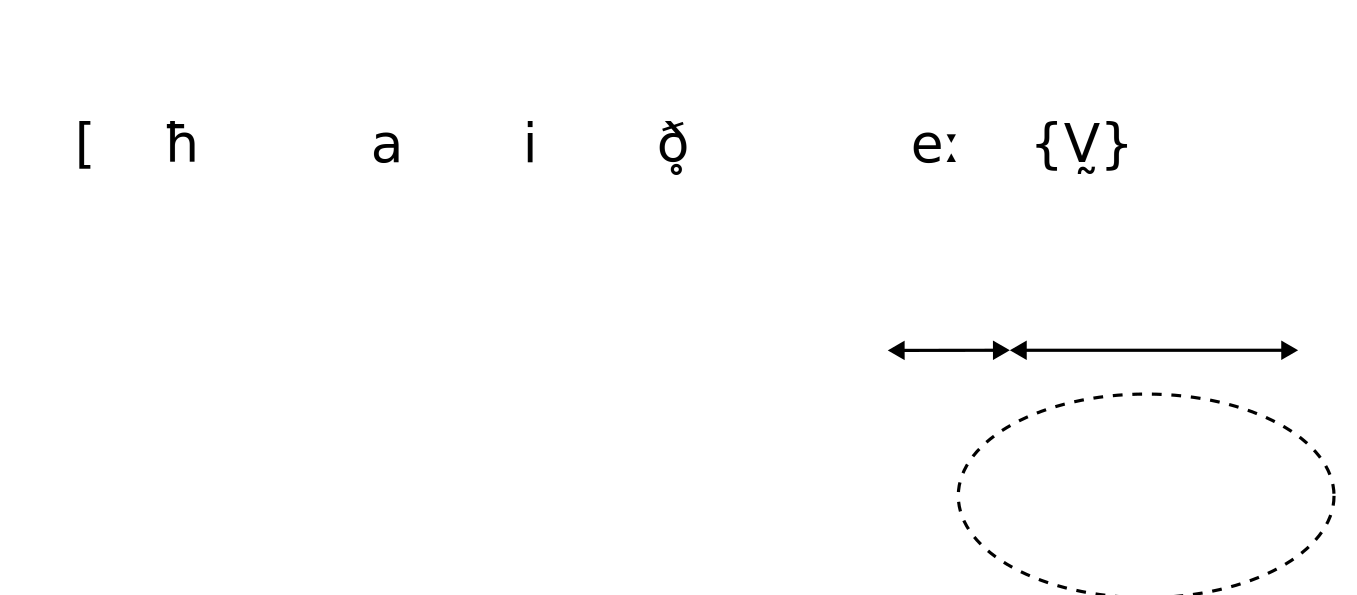
\includegraphics[height=.25\textheight]{figures/a12Watsonetal-img011.png}
}
\subfigure[\label{fig:watson:11b} Enlarged image of palates circled in \figref{fig:watson:11a}; measurement landmarks \textsc{onset} (frame \textsc{218),} \textsc{max} (frame 220) and \textsc{offset} (frame 236)]{
\includegraphics[height=.15\textheight]{figures/a12Watsonetal-img012.png}
}
\caption{\label{fig:watson:11} M001 \textit{ḥayḏēn} ‘the ear’ (Mehri)}
\end{figure}

\figref{fig:watson:11a} presents the synchronised waveform, spectrogram, palatogram and dynamic tongue-palate contact profile of an utterance-final \mbox{/n/} in Mehri realised with a silent alveolar articulation. The lines below the palatogram show alveolar contact (red line) and velar contact (blue line). The tongue-palate contact for the realisation of the \mbox{/n/} begins 86 ms after the end of the speaker’s final voice pulse. There is no evidence of any sound output during the time of the articulatory contact for the \mbox{/n/}, i.e. the \textsc{onset-offset} duration.

An enlarged image of the circled palate frames is given in \figref{fig:watson:11b}, enabling the reader to see the first contact of the tongue against the palate (frame 218), the maximum contact (frame 220), and the last contact before the articulation comes to an end (frame 236). Enlarged images of circled palate frames are also given for Figures~\ref{fig:watson:12}–\ref{fig:watson:14} below. Filled squares on the EPG palate frames represent areas of tongue contact; the top three rows represent the alveolar area, rows four and five the palatal area, and rows six to eight the velar area.

One bilingual speaker, J001, sometimes realises a final sonorant with voiceless noise which we take to be produced by a whisper setting, marked in the transcription as \{W\}. \figref{fig:watson:12} presents an example in which the vowel terminates in whispery-creak (marked as \{\{\Vdottilde{}\}) and glottal closure, with whisper starting when the glottal closure is released (release marked with an arrow on the spectrogram). The lateral articulation for the final \mbox{/l/} takes place during the whisper which has formant resonances approximately matching those of the sounded \mbox{/l/}; the auditory impression is of a whispered [ḷ].

\begin{figure}[p]
\subfigure[\label{fig:watson:12a} J001 \textit{ṣ̌lēl} ‘cross-eyed’ (Mehri) with aligned phonetic transcription; final \mbox{/l/}-articulation and dynamic tongue-palate contact profile circled on palatogram, glottal stop release arrowed on spectrogram; \textsc{onset} \textsc{delay} (143 ms) identified by double-headed arrow, \textsc{onset-offset} \textsc{(120} ms) by dashed double-headed arrow]{
\includegraphics[height=.25\textheight]{figures/a12Watsonetal-img013.pdf}
}
\subfigure[\label{fig:watson:12b} Enlarged image of palates circled in \figref{fig:watson:12a}; measurement landmarks \textsc{onset} (frame \textsc{78),} \textsc{max} (frame 84) and \textsc{offset} (frame 90)]{
\includegraphics[height=.15\textheight]{figures/a12Watsonetal-img014.png}
}
\caption{\label{fig:watson:12} J001 \textit{ṣ̌lēl} ‘cross-eyed’ (Mehri)}
\end{figure}

\begin{table}[p]
\caption{Duration values for \textsc{onset delay}, \textsc{onset-max} and \textsc{max-offset} for Shehret /l, n, r/; M=mean, SD=standard deviation, R=range}
\label{tab:watson:8}

\begin{tabularx}{\textwidth}{l@{~}rrrrrrrrr}
\lsptoprule
 & \multicolumn{3}{c}{\textsc{onset} \textsc{delay}} & \multicolumn{3}{c}{\textsc{onset-max}} & \multicolumn{3}{c}{\textsc{max-offset}}\\
 \cmidrule(lr){2-4}\cmidrule(lr){5-7}\cmidrule(lr){8-10}
& M & SD & R & M & SD & R & M & SD & R\\
\midrule
/l/ & 74.13 & 46.95 & 0-170 & 35.53 & 27.28 & 0-90 & 154.21 & 70.47 & 30-320\\
/n/ & 90.14 & 57.68 & 0-261 & 45.49 & 36.84 & 0-180 & 158.04 & 68.03 & 40-330\\
/r/ & 75.7 & 29.23 & 17-142 & 20.91 & 23.21 & 0-110 & 37.27 & 25.09 & 10-100\\
\lspbottomrule
\end{tabularx}
\end{table}

\subsubsection{Shehret unbreathed sonorants} %4.3.3 /
\label{sec:watson:4.3.3}

Our Shehret data set for utterance-final unbreathed sonorants in stressed syllables contained 134 tokens from three speakers (M026, J043, J001). The mean \textsc{onset} \textsc{delay}, \textsc{onset-max}, \textsc{max-offset} and \textsc{onset-offset} duration values with their ranges and standard deviations are given in \tabref{tab:watson:8} separately for \mbox{/l/}, \mbox{/n/} and \mbox{/r/}. Of the 134 tokens, three tokens of \mbox{/l/} and 2 of \mbox{/n/} show no onset delay. The remainder show delays of 50 ms or more in the majority of cases: 63\% of tokens in the case of \mbox{/l/} (mean onset delay 74 ms), 78\% for \mbox{/n/} (mean onset delay 90 ms), 84\% for \mbox{/r/} (mean onset delay 76 ms), with delays of 100 ms or more not uncommon: 26\% of tokens in the case of \mbox{/l/}, 39\% for \mbox{/n/}, and 23\% for \mbox{/r/}. These delay distributions are very similar to those for Mehri, except for \mbox{/r/} which has many more tokens of 100 ms or more in Mehri than in Shehret.\largerpage

The values are comparable to those in \tabref{tab:watson:7} for Mehri. Also comparable with Mehri is the extent and nature of variation within and across speakers with regard to the duration measures and the extent and location of articulatory contact during the silent realisations of the utterance-final sonorants, as can be seen in the figures below and in supplementary material.

As with the Mehri silent final \mbox{/l/} shown in \figref{fig:watson:1}, there is no acoustic output during the articulatory contact for final \mbox{/l/} in the Shehret word \textit{ṣ́ɛ̄l} in \figref{fig:watson:13}, nor is there any evidence of formant transitions in the vowel appropriate for a following alveolar consonant. Note that the articulatory contact is slightly retracted and less extensive along the lateral margins for the silent \mbox{/l/} than for the word-initial emphatic lateral fricative /ṣ́/.

\begin{figure}[p]
\subfigure[\label{fig:watson:13a} J043 \textit{ṣ́ɛ̄l} ‘cold’ (Shehret) with aligned phonetic transcription; silent articulation and dynamic tongue-palate contact profile circled on palatogram; \textsc{onset delay} (141 ms) identified by double-headed arrow, \textsc{onset-offset} \textsc{(160 ms}) by dashed double-headed arrow]{
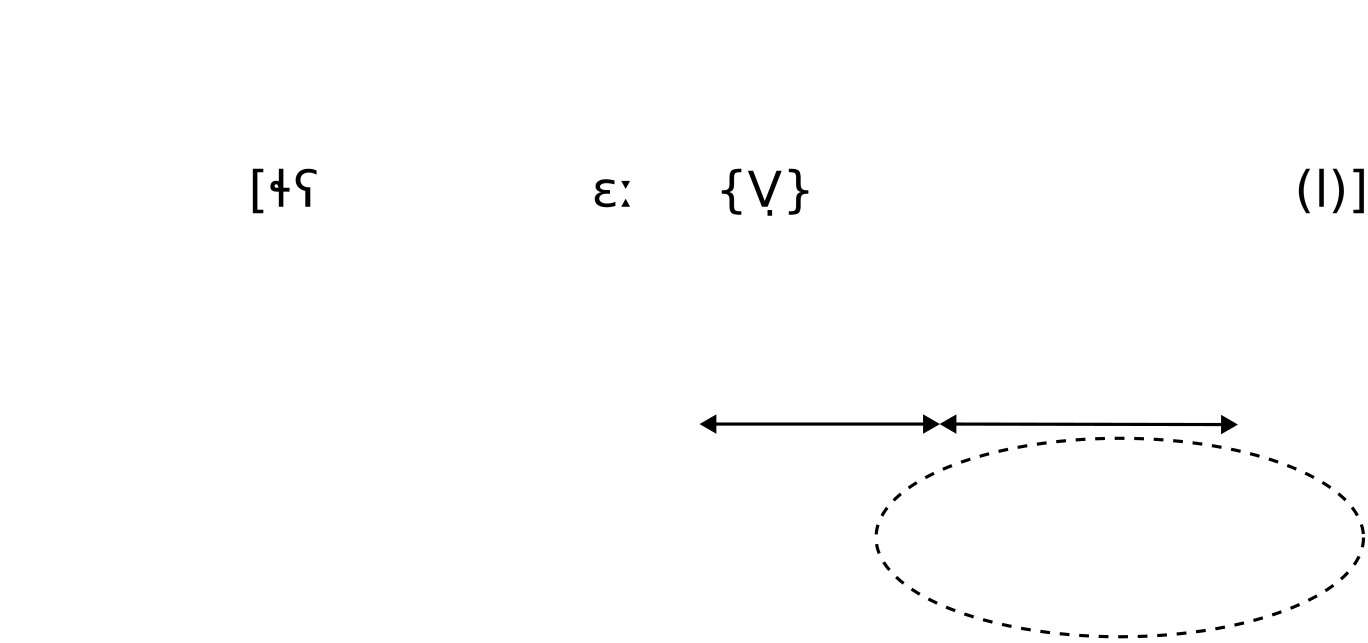
\includegraphics[height=.25\textheight]{figures/a12Watsonetal-img015.pdf}
}
\subfigure[\label{fig:watson:13b} Enlarged image of palates circled in \figref{fig:watson:13a}; measurement landmarks \textsc{onset} ({frame} \textsc{93),} \textsc{max} (frame 96) and \textsc{offset} (frame 109)]{
\includegraphics[height=.15\textheight]{figures/a12Watsonetal-img016.png}
}
\caption{\label{fig:watson:13} J043 \textit{ṣ́ɛ̄l} ‘cold’ (Shehret)}
\end{figure}

\begin{table}[p]
\caption{Duration values for \textsc{onset delay}, \textsc{onset-max} and \textsc{max-offset} for Shehret /ʰl, ʰn, ʰr/; M=mean, SD=standard deviation, R=range}
\label{tab:watson:9}

\begin{tabularx}{\textwidth}{l@{~}rrrrrrrrr}
\lsptoprule
 & \multicolumn{3}{c}{\textsc{onset} \textsc{delay}} & \multicolumn{3}{c}{\textsc{onset-max}} & \multicolumn{3}{c}{\textsc{max-offset}}\\
 \cmidrule(lr){2-4}\cmidrule(lr){5-7}\cmidrule(lr){8-10}
& M & SD & R & M & SD & R & M & SD & R\\
\midrule
/ʰl/ & 81.6 & 56.5 & 12-210 & 21.33 & 17.27 & 0-60 & 51.47 & 27.8 & 150-240\\
/ʰn/ & 141.31 & 76.47 & 21-470 & 51.37 & 55.32 & 0-320 & 110.0 & 66.16 & 40-280\\
/ʰr/ & 92.07 & 45.1 & 37-140 & 12.86 & 7.26 & 0-30 & 38.57 & 21.07 & 10-70\\
\lspbottomrule
\end{tabularx}
\end{table}

\subsubsection{Shehret breathed sonorants} %4.3.4 /
\label{sec:watson:4.3.4}
\largerpage
Our Shehret data set for utterance-final breathed sonorants contained 85 tokens from two speakers (M026, J043). The mean \textsc{onset} \textsc{delay}, \textsc{onset-max}, \textsc{max-off\-set} and \textsc{onset-offset} duration values with their ranges and standard deviations are given in \tabref{tab:watson:9} separately for \mbox{/ʰl/}, \mbox{/ʰn/} and \mbox{/ʰr/}. All tokens showed an onset delay which in the majority of cases reached 50 ms or more: 67\% of tokens in the case of \mbox{/ʰl/} (mean onset delay 82 ms), 96\% for \mbox{/ʰn/} (mean onset delay 141 ms), 71\% for \mbox{/ʰr/} (mean onset delay 92 ms). Delays of 100 ms or more are very common across all sonorants: 40\% of tokens in the case of \mbox{/ʰl/}, 73\% for \mbox{/ʰn/}, 57\% for \mbox{/ʰr/}.



The situation with respect to the breathed sonorants in Shehret is essentially the same as for the unbreathed sonorants, except that the vowel offset is marked by breathy voice (transcribed as \{V̤\}) and the onset delay typically contains some aspiration noise, shown by ʰ in \figref{fig:watson:14a}.

\begin{figure}
\subfigure[\label{fig:watson:14a} J043 \textit{ḥaʰl} ‘pressed oil’ (Shehret) with aligned phonetic transcription; silent articulation and dynamic tongue-palate contact profile circled on palatogram; \textsc{onset} \textsc{delay} (57 ms) identified by double-headed arrow, \textsc{onset-offset} (180 ms) by dashed double-headed arrow]{%
% 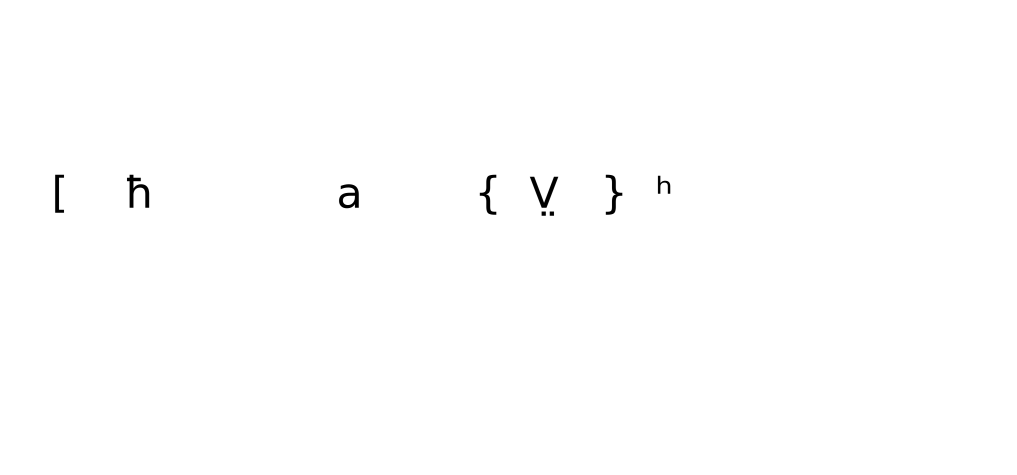
\includegraphics[width=\textwidth]{figures/a12Watsonetal-img017.pdf}
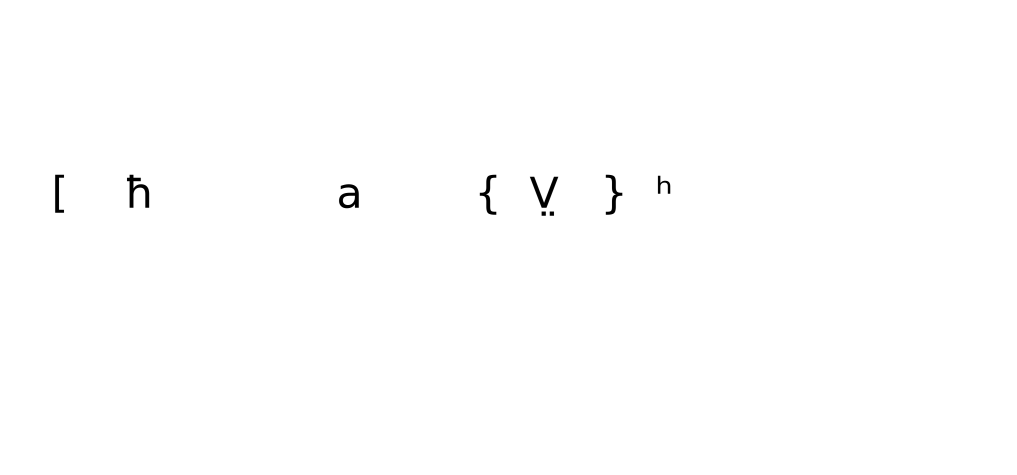
\includegraphics[height=.25\textheight]{figures/a12Watsonetal-img017.pdf}%
% [   ħ     a          \{   V̤  \}   ʰ                              (l) ]
}
\subfigure[\label{fig:watson:14b} Enlarged image of palates circled in \figref{fig:watson:14a}; measurement landmarks \textsc{onset} (frame \textsc{85),} \textsc{max} (frame 92) and \textsc{offset} (frame 103)]{\includegraphics[width=\linewidth]{figures/a12Watsonetal-img018.png}}
\caption{\label{fig:watson:14} J043 \textit{ḥaʰl} ‘pressed oil’ (Shehret)}
\end{figure}

\subsubsection{Summary of EPG results} %4.3.5 /
\label{sec:watson:4.3.5}
EPG methods were used to address RQs 1 and 2:

\begin{enumerate}
  \item Are utterance-final sonorants silent in careful speech?
  \item Are silent utterance-final sonorants articulated?
\end{enumerate}

Both of these questions are answered positively: lingual sonorants in utterance\hyp final position following a long vowel in Mehri and a full vowel in Shehret are all articulated with a gesture appropriate to the target sound and, with few exceptions, lack any accompanying acoustic signal. The non-silent exceptions are a few cases of \mbox{/r/}, and fewer of \mbox{/ʰr/}, due to the inherent nature of trilled articulation, and speaker J001’s whispered realisations. The lack of formant transitions in the preceding vowel and the lack of evidence of articulator activity during the onset delay provide justification for describing these sonorants as truly silent, a description corroborated by the informal test described in \sectref{sec:watson:5.3} in which a listener was unable to identify the final sonorant when the speaker’s back was turned.

Three phases can be identified in the time course of silent sonorants: the vowel offset, the onset delay, and the articulatory contact itself. The onset delay phase in the utterance-final sonorant data varies considerably in duration with a few tokens showing no delay but most showing delays of well over 50 ms, often extending to over 100 ms.

The articulatory contact phase also varies considerably both in how long it takes to form maximum articulatory contact (the \textsc{onset-max} measure), and in how long the contact remains in place (the \textsc{max-offset} measure), although the latter will be affected by the general phenomenon of pre-boundary lengthening whereby~segments immediately before certain boundaries are longer than those earlier in the utterance (\citealt{GussenhovenRietveld1992}). \textsc{Max-offset} values for \mbox{/r/} and \mbox{/ʰr/} are lower due to the prevalence of tap and trill realisations; these realisations also sometimes exhibit some brief voiceless turbulence.

In the case of unbreathed sonorants in both languages, the vowel offset is marked by creaky phonation; in the case of the Shehret breathed sonorants, it is marked by breathy voice. The onset delay phase is marked by silence in the case of pre-glottalised sonorants, but by aspiration in the case of the pre-aspirated ones. The vowel offset phase is explored further in \sectref{sec:watson:4.4}.

\subsection{Electrolaryngographic study} %4.4 /
\label{sec:watson:4.4}
This section examines collection and analysis methods of the ELG data, and then focuses on the analysis of three types of utterance-final segments: Mehri unbreathed sonorants, Shehret unbreathed sonorants, and Shehret breathed sonorants. The ELG study was designed to answer RQ 3:

\begin{enumerate}
  \item[3.] Does the larynx behave differently before silent utterance-final breathed sonorants than before silent utterance-final unbreathed sonorants?
\end{enumerate}

\subsubsection{Data collection and analysis} %4.4.1 /
\label{sec:watson:4.4.1}
ELG were recorded on a Laryngograph EGG-D200 microprocessor with an ECM 500L/SK lapel microphone both in the field in Dhofar between 2014 and 2021 and at the University of Leeds in 2015, 2017 and 2018. Closed quotient (CQ) values were taken at the mid-point and offset of the vowel preceding the utterance-final sonorant in a total of 781 tokens: 226 Mehri unbreathed sonorants, 226 Shehret unbreathed sonorants, 226 Shehret breathed sonorants, and 103 more Mehri tokens collected from speaker M001 whose results are presented separately in \sectref{sec:watson:4.4.6} due to their atypicality. In contrast to our EPG study, we are not investigating different places of articulation in the ELG study. We therefore present the data in \tabref{tab:watson:10} according to the number of unbreathed and breathed tokens recorded for each speaker rather than the number of individual segment tokens.

\begin{table}
\caption{Number of utterance-final silent sonorant tokens of each language by speaker for ELG analysis}
\label{tab:watson:10}
\begin{tabular}{lS[table-format=3.0] l S[table-format=3.0] S[table-format=3.0]}
\lsptoprule
 {Mehri} & {Unbreathed} & {Shehret} & {Unbreathed} & {Breathed}\\
 \midrule
 M001 & 103& J001 & 24 & 30\\
 M026 & 13 & J002 & 12 & 0\\
 M028 & 58 & J116 & 27 & 48\\
 M068 & 69 & J117 & 24 & 19\\
 M079 & 70 & J028 & 27 & 48\\
 J001 & 16 & J043 & 95 & 63\\
      &    & M026 & 17 & 18\\
\midrule
 Total & {329} & Total & {226} & {226}\\
\lspbottomrule
\end{tabular}
\end{table}

The closed quotient (CQ) of a glottal voicing cycle is the proportion of the cycle during which the vocal folds are in contact, expressed as a percentage of the whole cycle (\citealt{AbbertonFourcin1989}: 290). The lower the CQ value of a cycle, the more air is free to flow through the glottis. There is thus an inverse relation between CQ and transglottal airflow, with values below about 40\% tending to sound increasingly breathy (\citealt{HeselwoodMaghrabi2015}: 153–154; \citealt{WrightEtAl2019} give 34\% as typifying breathy voice). The voice quality of a vowel typically shows coarticulatory effects depending on the glottal state of the adjacent consonant (\citealt{GoblChasaide1999}). Open-glottis consonants prompt lower CQ values at vowel edges in contrast to voiced consonants and consonants with the glottis in what \citet[356]{EslingHarris2005} call a constricted ``prephonation'' state as found,
for example, at the release of unaspirated stops. By taking CQ values at the offsets of vowels we can therefore gain information about the relative size of the glottal opening at the start of the following consonant and the extent to which it impedes or facilitates transglottal airflow. Comparison with the CQ value at the vowel’s mid-point reveals whether the glottis is becoming increasingly unconstructed, and hence increasingly open, as the vowel approaches the following consonant or not. Aspirated (breathed) segments are produced with an open glottis, while unaspirated (unbreathed) are produced with a more closed glottis. We therefore predict that Shehret breathed sonorants will exhibit CQ values below 40\% and Mehri and Shehret unbreathed sonorants will exhibit CQ values above 40\%.

The two measurement CQ landmarks are the glottal cycle at the mid-point of the vowel, which we take to be half-way along the train of glottal pulses,\footnote{We measure half-way along the train of glottal pulses rather than the mid-point of the vowel, as the number of glottal pulses is less arbitrary than an estimate of vowel duration.} and the final regular glottal cycle at the vowel offset. Irregular cycles were excluded because of the risk of inaccuracies due to double pulsing and very long glottal closed phases.

CQ values were assigned to bins on a 0–100\% scale, as given in Figures~\ref{fig:watson:15},~\ref{fig:watson:19}, and~\ref{fig:watson:22}. The significant divide is at around 40\%.

\subsubsection{Mehri unbreathed sonorants} %4.4.2 /
\begin{figure}[b]
% \includegraphics[width=\textwidth]{figures/a12Watsonetal-img019.png}
\begin{tikzpicture}
\begin{axis}[
    width  = \textwidth,
    height  = .3\textheight,
    axis lines*=left,
    ybar,
    ymin=0,
    ymax=90,
    ylabel={Number of tokens},
    xlabel={Distribution bins},
    symbolic x coords={0-19,20-24,25-29,30-34,35-39,40-44,45-49,50-54,55-59,60+},
    xtick=data
    ]
\addplot[black,fill=gray] coordinates {
(0-19,0)
(20-24,0)
(25-29,0)
(30-34,1)
(35-39,7)
(40-44,38)
(45-49,80)
(50-54,58)
(55-59,37)
(60+,5)
};
\end{axis}
\end{tikzpicture}
\caption{Distribution of CQ values at vowel offset before final silent sonorants in Mehri}
\label{fig:watson:15}
\end{figure}

\label{sec:watson:4.4.2}
\figref{fig:watson:15} presents the distribution of CQ values for vowel offsets in Mehri (excluding atypical speaker M001) before silent sonorants. 80\% of values are in the 45\%+ range, with only 4\% falling below 40\%. From this we can conclude that the glottis does not begin to open during the final part of the vowel, a conclusion consistent with the creaky phonation seen in the spectrograms below and in \sectref{sec:watson:4.1}. \figref{fig:watson:16} shows that averaged across all tokens there is virtually no change in CQ value from vowel mid-point to vowel offset, the slope being almost level.


  
\begin{figure}
% \includegraphics[width=\textwidth]{figures/a12Watsonetal-img020.png}
% \includegraphics[width=\textwidth]{figures/a12Watsonetal-img020.svm}
\begin{tikzpicture}
  \begin{axis}[
    height  = .3\textheight,
    width=8cm,
    axis lines*=left,
    ymin=0,
    ymax=60,
    xlabel={CQ sample point},
    ylabel={\% CQ},
    ylabel near ticks,
    enlarge x limits=0.5,
    xtick=data,
    nodes near coords,
    symbolic x coords={
        ignore,
        V mid-point,
        V-offset,
        ignore2
      }
    ]
\addplot[black,mark=*] plot coordinates {(V mid-point,50.12) (V-offset,49)};
\end{axis}
\end{tikzpicture}
\caption{Averaged CQ slope from vowel mid-point to vowel offset before final silent sonorants in Mehri}
\label{fig:watson:16}
\end{figure}

The following figures present examples of the sonorant consonants /l, r/ in Mehri. Figures presenting examples of /n, m/ are provided in supplementary material. The figures show little change in CQ value from the vowel mid-point to vowel offset, closely replicating the slope of the averaged values in \figref{fig:watson:16}. \figref{fig:watson:17} shows synchronized spectrogram, audio waveform (blue), larynx waveform (green) and CQ trace (pink line) for the second syllable of \textit{ṯīḳōl.} The larynx waveform represents the alternate closing and opening of the vocal folds during voicing: the waveform peaks represent maximum closure, the valleys represent maximum opening. In this figure, the CQ slope remains relatively flat during the vowel in the 45–49\% range with the final few pulses showing evidence of creaky phonation. The final \mbox{/l/} is silent.

\begin{figure}[t]
\includegraphics[width=\textwidth]{figures/a12Watsonetal-img021.pdf}
% [  k’                                        oː                     \{     V̰     \}         (l)]
\caption{M028 \textit{(ṯī)ḳōl} ‘heavy.\textsc{m.pl}’ with aligned phonetic transcription; CQ at mid-point = 48\% (arrowed), CQ at offset = 48\% (at cursor)}
\label{fig:watson:17}
\end{figure}

In \figref{fig:watson:18}, the CQ value rises from 50\% at vowel mid-point to 55\% at the offset of the vowel preceding final \mbox{/r/} in Mehri \textit{āfōr} ‘clouds’. Note that \mbox{/r/} is realised as a two-beat devoiced trill after a silent onset delay of 162 ms.\footnote{Also worthy of note is that \mbox{/f/} is realised with breathy voice with a CQ value reaching as low as 21\% in this instance; that is to say, it is phonetically voiced while remaining phonologically ``breathed''.}

\begin{figure}
\includegraphics[width=\textwidth]{figures/a12Watsonetal-img022.pdf}
% [ aː                f             oː                                  r̥ ]
\caption{M068 \textit{āfōr} ‘clouds’ (Mehri) with aligned phonetic transcription; CQ=50\% at mid-point (arrowed), 55\% at offset (at cursor)}
\label{fig:watson:18}
\end{figure}

\subsubsection{Shehret unbreathed sonorants} %4.4.3 /
\label{sec:watson:4.4.3}
\figref{fig:watson:19} presents the distribution of CQ values for vowel offsets in Shehret before silent unbreathed sonorants. The values are more spread out than they are in Mehri, although the general pattern is similar, with 12\% exhibiting CQ values below 40\%. Of the rest, 78\% have CQs of 45\% or above. \figref{fig:watson:20} shows on average the CQ slope is almost flat, however, as was the case in the Mehri data.

\begin{figure}[t]
% \includegraphics[width=\textwidth]{figures/a12Watsonetal-img023.svm}
% \includegraphics[width=\textwidth]{figures/a12Watsonetal-img023.png}
\begin{tikzpicture}
\begin{axis}[
    width  = \textwidth,
    height  = .3\textheight,
    axis lines*=left,
    ybar,
    ymin=0,
    ymax=90,
    ylabel={Number of tokens},
    xlabel={Distribution bins},
    symbolic x coords={0-19,20-24,25-29,30-34,35-39,40-44,45-49,50-54,55-59,60+},
    xtick=data
    ]
\addplot[lsDarkOrange,fill=lsMidOrange] coordinates {
(0-19,0)
(20-24,2)
(25-29,1)
(30-34,11)
(35-39,13)
(40-44,23)
(45-49,38)
(50-54,61)
(55-59,60)
(60+,17)
};
\end{axis}
\end{tikzpicture}
% 0
% 2
% 1
% 11
% 13
% 23
% 38
% 61
% 60
% 17
\caption{Distribution of CQ values at vowel offset before final silent unbreathed sonorants in Shehret}
\label{fig:watson:19}
\end{figure}

\begin{figure}[p]
% \includegraphics[width=\textwidth]{figures/a12Watsonetal-img024.svm}
% \includegraphics[width=\textwidth]{figures/a12Watsonetal-img024.png}
\begin{tikzpicture}
  \begin{axis}[
    height  = .3\textheight,
    width=8cm,
    axis lines*=left,
    ymin=0,
    ymax=60,
    xlabel=CQ sample point,
    ylabel=\% CQ,
    ylabel near ticks,
    xtick=data,
    enlarge x limits = 0.5,
    nodes near coords,
    symbolic x coords={V mid-point,V-offset}
    ]
\addplot[orange,mark=*] plot coordinates {
    (V mid-point,49.33)
    (V-offset,50.52)
};
\end{axis}
\end{tikzpicture}
\caption{Averaged CQ slope from vowel mid-point to vowel offset before final silent unbreathed sonorants in Shehret}
\label{fig:watson:20}
\end{figure}

\figref{fig:watson:21} presents the spectrogram, audio waveform, larynx waveform and CQ trace of final unbreathed \mbox{/l/} in Shehret. Figures in supplementary material present examples for each of the other unbreathed sonorants /m, n, r/. As with the Mehri examples, the CQ slopes in some remain relatively flat, while they rise slightly in others.

\begin{figure}[p]
% 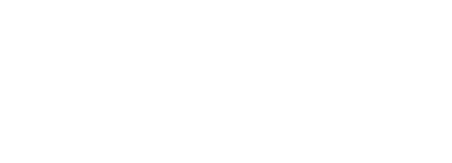
\includegraphics[width=\textwidth]{figures/a12Watsonetal-img025.png}
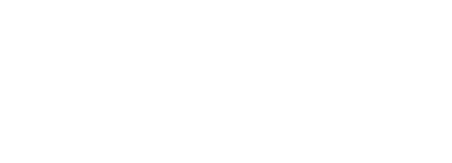
\includegraphics[width=\textwidth]{figures/a12Watsonetal-img025.pdf}
%    [ ɮ           iː        j      ɛ  \{ V̰ \}                (l) ]
\caption{J043 \textit{źīyɛl} ‘camel herders’ (Shehret) with aligned phonetic transcription; CQ=54\% at mid-point (arrowed), 61\% at offset (at cursor); position of silent \mbox{/l/} very approximate}
\label{fig:watson:21}
\end{figure}

\subsubsection{Shehret breathed sonorants} %4.4.4 /
\label{sec:watson:4.4.4}

\begin{figure}[p]
% \includegraphics[width=\textwidth]{figures/a12Watsonetal-img026.svm}
% \includegraphics[width=\textwidth]{figures/a12Watsonetal-img026.png}
\begin{tikzpicture}
\begin{axis}[
    width  = \textwidth,
    height  = .3\textheight,
    axis lines*=left,
    ybar,
    ymin=0,
    ymax=90,
    ylabel={Number of tokens},
    xlabel={Distribution bins},
    symbolic x coords={0-19,20-24,25-29,30-34,35-39,40-44,45-49,50-54,55-59,60+},
    xtick=data
    ]
    \addplot+[lsDarkBlue,fill=lsMidBlue] coordinates {
(0-19,53)
(20-24,78)
(25-29,48)
(30-34,33)
(35-39,9)
(40-44,5)
(45-49,0)
(50-54,0)
(55-59,0)
(60+,0)
};
\end{axis}
\end{tikzpicture}
\caption{Distribution of CQ values at vowel offset before final silent breathed sonorants in Shehret}
\label{fig:watson:22}
\end{figure}

The distribution of CQ values for vowel offsets in Shehret before silent breathed sonorants is presented in \figref{fig:watson:22}. Only five tokens (2\%) had a CQ of 40\% or more, and 79\% had CQ values below 30\%, well within the range for breathy voice phonation. In marked contrast to the vowels before the unbreathed sonorants in both Shehret and Mehri, \figref{fig:watson:23} shows that, on average, the CQ slope of a vowel drops 23\% before a breathed sonorant. The indication is, therefore, that the glottis becomes less constricted towards the end of the vowel in anticipation of its opening to allow voiceless air to flow through in the form of aspiration.


\begin{figure}
% \includegraphics[width=\textwidth]{figures/a12Watsonetal-img027.svm}
% \includegraphics[width=\textwidth]{figures/a12Watsonetal-img027.png}
\begin{tikzpicture}
  \begin{axis}[
    height  = .3\textheight,
    width=8cm,
    axis lines*=left,
    ymin=0,
    ymax=60,
    xlabel=CQ sample point,
    ylabel=\% CQ,
    ylabel near ticks,
    nodes near coords,
    xtick=data,
    enlarge x limits = 0.5,
    symbolic x coords={
        V mid-point,
        V-offset
      }
    ]
\addplot[blue,mark=*] plot coordinates {
    (V mid-point,46.78)
    (V-offset,24.17)
};
\end{axis}
\end{tikzpicture}
\caption{\label{fig:watson:23} Averaged CQ slope from vowel mid-point to vowel offset before final silent breathed sonorants in Shehret}
\end{figure}

ELG data of the breathed sonorants /ʰl, ʰm, ʰn, ʰr/ in Shehret show an average fall in the CQ slope from the vowel mid-point to a value below 30\% at vowel offset. These falls are not observed in the data for the unbreathed sonorants in either Shehret or Mehri (although see \sectref{sec:watson:4.4.6}). They indicate that the vocal folds are undergoing a progressive reduction in contact during subsequent cycles of voicing preparatory to the appearance of aspiration which can be seen on the spectrograms as soon as voicing ceases. \figref{fig:watson:24} provides an example of \mbox{/ʰl/}, taking the final syllable from (\textit{eg})\textit{miʰl} ‘the camels’. Further figures and discussion are available in the supplementary material.

\begin{figure}[t]
% 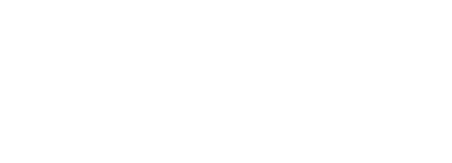
\includegraphics[width=\textwidth]{figures/a12Watsonetal-img028.png}
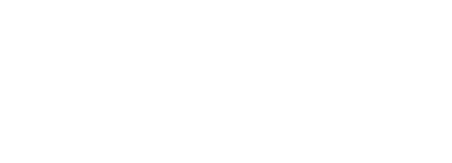
\includegraphics[width=\textwidth]{figures/a12Watsonetal-img028.pdf}
% [ m                                 i               ʰ              (l) ]
\caption{J001 (\textit{eg})\textit{miʰl} ‘the camels’ (Shehret) with aligned phonetic transcription; CQ=50\% at mid-point (arrowed), 20\% at offset (at cursor); position of silent \mbox{/l/} very approximate}
\label{fig:watson:24}
\end{figure}

\subsubsection{Summary of ELG results} %4.4.5 /
\label{sec:watson:4.4.5}
ELG methods were used to address RQ 3:

\begin{enumerate}
  \item[3.] Does the larynx behave differently before utterance-final breathed sonorants than before utterance-final unbreathed sonorants?
\end{enumerate}

For convenience of comparison, Figures \ref{fig:watson:15}, \ref{fig:watson:19} and \ref{fig:watson:22} are combined in \figref{fig:watson:25} where it can easily be seen that vowel offset CQ values for Mehri and Shehret unbreathed sonorants have very similar distributions in clear contrast to those for Shehret breathed sonorants. Figures \ref{fig:watson:16}, \ref{fig:watson:20} and \ref{fig:watson:23} are combined in \figref{fig:watson:26} to show that on average CQ slopes remain almost level well above 40\% for Mehri and Shehret unbreathed sonorants, but fall quite steeply to well below 30\% for Shehret breathed sonorants.

\begin{figure}[t]
% \includegraphics[width=\textwidth]{figures/a12Watsonetal-img029.svm}
% \includegraphics[width=\textwidth]{figures/a12Watsonetal-img029.png}
\begin{tikzpicture}
\begin{axis}[
    width  = \textwidth,
    height  = .3\textheight,
    axis lines*=left,
    ybar,
    ymin=0,
    ymax=90,
    bar width=5pt,
    ymajorgrids,
    ylabel={Number of tokens},
    xlabel={Distribution bins},
    ylabel near ticks,
    symbolic x coords={0-19,20-24,25-29,30-34,35-39,40-44,45-49,50-54,55-59,60+},
    xtick=data,
    legend style={at={(0.5,1)}, anchor=south},
    legend columns=3,
    ]
\addplot+[lsDarkBlue,fill=lsMidBlue] coordinates {
(0-19,53)
(20-24,78)
(25-29,48)
(30-34,33)
(35-39,9)
(40-44,5)
(45-49,0)
(50-54,0)
(55-59,0)
(60+,0)
};
\addplot+[lsDarkOrange,fill=lsMidOrange] coordinates {
(0-19,0)
(20-24,0)
(25-29,1)
(30-34,11)
(35-39,13)
(40-44,23)
(45-49,38)
(50-54,61)
(55-59,60)
(60+,17)
};
\addplot+[black,fill=gray] coordinates {
(0-19,0)
(20-24,0)
(25-29,0)
(30-34,1)
(35-39,7)
(40-44,38)
(45-49,80)
(50-54,58)
(55-59,37)
(60+,5)
};
\legend{Shehret breathed, Shehret unbreathed, Mehri}
\end{axis}
\end{tikzpicture}
% 53  0   0
% 78  0   0
% 48  1   0
% 33  11  1
% 9   13  7
% 5   23  38
% 0   38  80
% 0   61  58
% 0   60  37
% 0   17  5
% \todo[inline]{check data}

% \todo[inline]{check values}
\caption{Comparison of distribution of CQ values at vowel offset before final silent sonorants in Mehri and Shehret}
\label{fig:watson:25}
\end{figure}

\begin{figure}
% \includegraphics[width=\textwidth]{figures/a12Watsonetal-img030.svm}
% \includegraphics[width=\textwidth]{figures/a12Watsonetal-img030.png}
\begin{tikzpicture}
\begin{axis}[
    axis lines*=left,
    height = .3\textheight,
    width=8cm,
    enlarge x limits={0.55},
    ymin=0,
    ymax=55,
    xlabel=CQ sample point,
    ylabel=\% CQ,
    ylabel near ticks,
    xtick=data,
    symbolic x coords={Vowel mid-point,Vowel offset},
    legend pos={outer north east},
    legend cell align=left
    ]
    \addplot[lsMidBlue,mark=*,nodes near coords, 
             nodes near coords align={below}] plot coordinates {
        (Vowel mid-point,46.78)
        (Vowel offset,24.17)
    };
    \addlegendentry{Shehret breathed}
    \addplot[lsMidOrange,mark=*,
             every pin edge/.style={lsMidOrange}] plot coordinates {
        (Vowel mid-point,49.33)
        (Vowel offset,50.52)
    }
    % Instead of "nodes near coords", manually place pins
    node [pos=0, pin=180:49.33, pin distance=.5ex] {}
    node [pos=1, pin=0:50.52, pin distance=.5ex] {};
    \addlegendentry{Shehret unbreathed}
    \addplot[black,mark=*,nodes near coords] plot coordinates {
        (Vowel mid-point,50.12)
        (Vowel offset,49)
    };
    \addlegendentry{Mehri}
\end{axis}
\end{tikzpicture}
% \todo[inline]{please decide which of (un)breathed should be blue/orange}
\caption{Comparison of averaged CQ slopes in Mehri and Shehret (Shehret unbreathed line partially obscured by Mehri line)}
\label{fig:watson:26}
\end{figure}

The ELG results answer RQ 3 positively: {the larynx does behave differently before utterance-final breathed sonorants than before utterance-final unbreathed sonorants.} The ELG results provide evidence of the behaviour of the glottis during the vowel offset phase of final silent sonorants in both languages, showing that the glottis is relatively constricted prior to the onset delay phase of unbreathed sonorants, but becomes increasingly unconstricted prior to the onset delay phase of the Shehret breathed sonorants. This difference in glottal constriction at vowel offset results in the onset delay phase being silent in unbreathed sonorants due to lack of transglottal airflow, but noisy for at least the first part of the onset delay phase in Shehret breathed sonorants due to transglottal airflow being facilitated.

\subsubsection{Simultaneous pre-glottalisation and pre-aspiration} %4.4.6 /
\label{sec:watson:4.4.6}
We have so far excluded one speaker (M001) in our Mehri data because of his atypically and exceptionally low CQ values for all vowel tokens at vowel offset. His CQ distribution is shown in \figref{fig:watson:27}, his averaged CQ slope can be seen in \figref{fig:watson:28}, and an example of his production of the word \textit{yiṣ́lēl} in \figref{fig:watson:29}. From these figures, it can be seen how similar his CQ values are to those associated with the breathed sonorants in Shehret.\largerpage

\begin{figure}
% \includegraphics[width=\textwidth]{figures/./ObjectReplacements/Object 10}
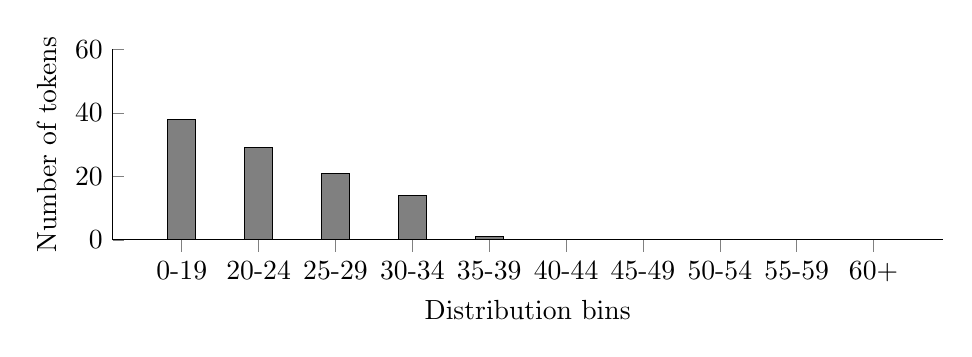
\begin{tikzpicture}
\begin{axis}[
    width  = \textwidth,
    height  = 4cm,
    axis lines*=left,
    ybar,
    ymin=0,
    ymax=60,
    ylabel={Number of tokens},
    xlabel={Distribution bins},
    symbolic x coords={0-19,20-24,25-29,30-34,35-39,40-44,45-49,50-54,55-59,60+},
    xtick=data
    ]
\addplot[black,fill=gray] coordinates {
(0-19,38)
(20-24,29)
(25-29,21)
(30-34,14)
(35-39,1)
(40-44,0)
(45-49,0)
(50-54,0)
(55-59,0)
(60+,0)
};
\end{axis}
\end{tikzpicture}
\caption{Distribution of speaker M001’s CQ values at vowel offset before final silent sonorants in Mehri}
\label{fig:watson:27}
\end{figure}

\begin{figure}
% \includegraphics[width=\textwidth]{figures/a12Watsonetal-img031.svm}
% \includegraphics[width=\textwidth]{figures/a12Watsonetal-img031.png}
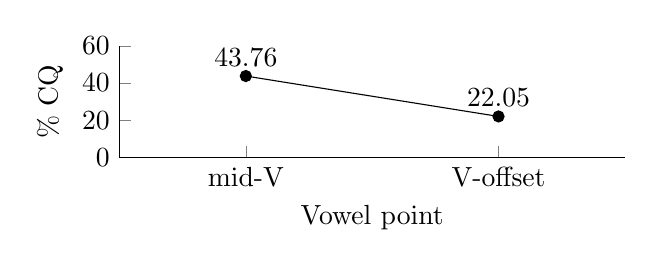
\begin{tikzpicture}
  \begin{axis}[
    height  = 3cm,
    width=8cm,
    axis lines*=left,
    ymin=0,
    ymax=60,
    xlabel=Vowel point,
    ylabel=\% CQ,
    ylabel near ticks,
    xtick=data,
    enlarge x limits = 0.5,
    nodes near coords,
    symbolic x coords={mid-V,V-offset}
    ]
\addplot[black,mark=*] plot coordinates {(mid-V,43.76) (V-offset,22.05)};
\end{axis}
\end{tikzpicture}

\caption{Averaged CQ slope from vowel mid-point to vowel offset before final silent sonorants in Mehri for speaker M001}
\label{fig:watson:28}
\end{figure}

\begin{figure}

% \includegraphics[width=\textwidth]{figures/a12Watsonetal-img032.png}

\includegraphics[width=\textwidth]{figures/a12Watsonetal-img032.pdf}

% [ l                    eː     \{  V̰̣  \}              ʔ                                  (l) ]
\caption{M001 (\textit{yiṣ́})\textit{lēl} ‘he goes wrong’ (Mehri) with aligned phonetic transcription; CQ=50\% at mid-point (arrowed), 25\% at offset (at cursor); glottal release arrowed; position of silent \mbox{/l/} very approximate}
\label{fig:watson:29}
\end{figure}

The resemblance of M001’s vowel offsets to those preceding pre-aspirated sonorants looks on the face of it to run counter to what the other Mehri speakers’ CQ values lead us to expect in terms of glottal constriction, but closer inspection may provide an explanation. \citeauthor{Hejná2022} (\citeyear*{Hejná2022}, see also \citetv{chapters/16_Hejná}) concludes from a study of Welsh-accented English that pre-glottalisation does not preclude pre-aspiration and that both can occur together manifesting as whispery creak. The creak pulses evident in the spectrogram in \figref{fig:watson:29} together with the falling CQ values suggest that M001 may be employing whispery creak phonation (marked on the transcription as \{\Vdottilde{}\}, with subscript dot beneath tilde) at the offset of vowels before final silent sonorants: the whisper is visible on the relevant spectrograms for this speaker; however, the auditory impression is of a glottal stop at the end of the vowel, and a glottal release can be seen on the spectrogram (arrowed). The posterior opening of the glottis for the whisper component of whispery creak \citep[100]{Catford1977} will be responsible for the low CQ values, and the anterior medial compression responsible for the creakiness. The whisperiness itself may result from sphinctering of the aryepiglottic folds (\citealt{EslingHarris2005}: 367; \citealt{MoisikEtAl2019}). It is also significant in view of our ``breathed–unbreathed'' analysis of Mehri and Shehret laryngeal phonology that airflow is lower during whisper settings than during breathy voice (\citealt{EslingHarris2005}: 368).

\section{Discussion} %5. /
\label{sec:watson:5}
\largerpage
This section is divided into a summary of results (\sectref{sec:watson:5.1}), a discussion of laryngeal categories (\sectref{sec:watson:5.2}), a discussion of how silently articulated sonorants can be incorporated into the literature on lenition (\sectref{sec:watson:5.3}), and further research (\sectref{sec:watson:5.4}).

\subsection{Summary of results} %5.1 /
\label{sec:watson:5.1}
In our EPG data, utterance-final singleton sonorant consonants in a stressed syllable are always realized with an articulation, which is typically silent, in both languages. In Mehri, utterance-final geminate sonorants are fully sounded with voicing in the initial portion without pre-glottalisation or pre-aspiration, as are many, but not all, singleton sonorants in post-tonic syllables. The absence of sound can be seen in almost all the examples we present in this chapter and in supplementary material, and is underscored by the comment from M001 that were a speaker to voice a singleton sonorant in an utterance-final stressed syllable listeners would find it comical. There may therefore be social pressure not to voice them. M001 was equally insistent that, despite its silence, the articulation of a final sonorant is always executed, a claim borne out by our data. One bilingual speaker, J001, however, realises his final unbreathed sonorants with whisper phonation in a minority of cases, an example of which is presented in \figref{fig:watson:12}. Very occasionally, some light noise is evident after the offset of a silent articulation which we take to be turbulent air exiting through the channel opened by the articulatory release.

The atypical laryngeal behaviour of M001 discussed in~\sectref{sec:watson:4.4.6}, we believe, may be partly due to the fact that there is no contrast in Mehri between unbreathed and breathed sonorants; there is therefore less need for Mehri speakers than for Shehret speakers to produce significantly higher CQ values in this context providing there is some form of pre-glottalisation.

The phonatory component of final sonorants, however, is generally not completely silent if we take modulations to the offset of the preceding vowel as evidence of phonatory co-production. In the case of the unbreathed sonorants of Mehri and Shehret, this takes the form of creaky phonation. In the case of the breathed sonorants of Shehret, it takes the form of breathy voice followed by aperiodic noise. Whether or not these modulations function as perceptual cues is a question we have to leave open in the absence of experimental evidence. In some tokens, there is also a detectable manner-of-articulation cue in the form of degrees of nasalisation on a vowel preceding a silently articulated nasal.

\subsection{Laryngeal categories} %5.2 /
\label{sec:watson:5.2}
As discussed in \sectref{sec:watson:2.5}, voiced and emphatic consonants share phonetic and morphophonological characteristics (\citealt{WatsonHeselwood2016}), motivating the shared laryngeal feature ``unbreathed'' as opposed to ``breathed'' for voiceless consonants. As noted in \sectref{sec:watson:4.4.5}, many tokens of utterance-final unbreathed sonorants show creaky phonation at vowel offset. These tokens, and many that do not show creaky phonation, give the auditory impression of terminating in a complete glottal closure. Evidence of glottal release occurring during the onset delay phase of final silent unbreathed sonorants from our EPG data can be seen in \figref{fig:watson:12}, and from our ELG data in \figref{fig:watson:17} and \figref{fig:watson:29}. The fact that unbreathed sonorants exhibit pre-glottalisation and relatively high CQ values in preceding vowel offsets, and that breathed sonorants exhibit pre-aspiration and much lower CQ values in preceding vowel offsets, supports the ``unbreathed'' vs. ``breathed'' analysis of their laryngeal behaviour referred to in \sectref{sec:watson:2.5}. The terms of the analysis derive from focusing on the breath-controlling function of the glottis rather than the tone-generating function (\citealt{HeselwoodWatson2021}). Further research into the behaviour of the larynx in Mehri and Shehret would benefit greatly from laryngoscopic and aerometric investigation.

\begin{figure}[b]
\subfigure[voiceless]{
\includegraphics[height=.2\textheight]{figures/a12Watsonetal-img033.pdf}
}
\subfigure[emphatic]{
\includegraphics[height=.2\textheight]{figures/a12Watsonetal-img034.pdf}
}
\subfigure[voiced]{
\includegraphics[height=.2\textheight]{figures/a12Watsonetal-img035.pdf}
}
\caption{J001 utterance-final (a) voiceless, (b) emphatic and (c) voiced alveolar stops (Mehri); note the articulation onset delay in the emphatic and voiced stops but not the voiceless stop}
\label{fig:watson:30}
\end{figure}

The glottalised vowel offset and silent onset delay before unbreathed sonorants is also observed in our EPG data before utterance-final emphatic and voiced obstruents in both languages.\footnote{For Shehret, \citet{HeselwoodEtAl2022} report mean gap durations of 60 ms before final emphatic fricatives, 109 ms before voiced fricatives, and no gap before voiceless fricatives.} Examples are shown in \figref{fig:watson:30} for the voiceless\hyp emphatic\hyp voiced triad of alveolar stops in Mehri, and in \figref{fig:watson:31} for the fricative voiceless-emphatic-voiced triad in Shehret. The lack of glottalisation or onset delay before voiceless consonants means that, in the case of fricatives, friction noise follows immediately on from the vowel thus paralleling the aspiration in pre-aspirated sonorants which also follows immediately on from the vowel. This similarity again justifies placing pre-aspirated sonorants in the same laryngeal class as voiceless obstruents, and plain sonorants in the same class as emphatic and voiced obstruents.



\begin{figure}[t]
\subfigure[voiceless]{
\includegraphics[height=.16\textheight]{figures/a12Watsonetal-img036.pdf}
}
\subfigure[emphatic]{
\includegraphics[height=.16\textheight]{figures/a12Watsonetal-img037.pdf}
}
\subfigure[voiced]{
\includegraphics[height=.16\textheight]{figures/a12Watsonetal-img038.pdf}
}
\caption{J043 utterance-final (a) voiceless, (b) emphatic and (c) voiced alveolar fricatives and their realisations (Shehret); note the glottalised offset, onset delay and acoustic gap in the emphatic and voiced fricatives, but not the voiceless fricative which has a breathy offset}
\label{fig:watson:31}
\end{figure}

Although place distinctions are lost acoustically among utterance-final sonorants, the stop–fricative–sonorant manner contrast is maintained by the respective phonetic exponents ``burst''–``friction''–``silence''.

\subsection{{Lenition}}\label{sec:watson:5.3}
Sonorants have rarely been examined within the recent literature on lenition, one exception being the work of \citet{LawsonEtAl2015} on lenited final \mbox{/r/} in Scottish English; however, final sonorants are prone to significant synchronic and diachronic instability, typically becoming more vowel-like and moving up the sonority scale. This includes vocalisation of \mbox{/l/} and \mbox{/r/} in varieties of English (\citealt{Wells1982} for \textit{l}-vocalisation; \citealt{Lutz1994} for \textit{r}-vocalisation), Romance and Germanic, a process which has resulted in the diachronic loss of \mbox{/l/} in certain words in Dutch, as in \textit{goud} ‘gold’ but \textit{gulden} ‘golden’, and in French, as in \textit{chaud} ‘hot’ from Vulgar Latin \textit{caldu(m)}, \textit{l-}vocalisation in Mehri (\citealt{Rubin2014}; \citealt{WatsonEtAl2020}) and Shehret \citep{Rubin2014}, loss of nasals with nasalisation of the preceding vowel in French \citep{Rochet1976} and Portuguese \citep{Cruz-Ferreira1995}, and anticipatory assimilation of sonorants in Arabic \citep{Watson2002}.

{We assume that utterance-final silent sonorants fall in the category of consonant lenition. \citet[265]{Harris1990} describes lenition as ``a reduction in the complexity of a segment'', and this is indeed what we find in our data. Utterance-final position is one of the conditioning environments for lenition \citep[8]{Kirchner1998}. The typical cline of lenition is given below (after \citealt{Guravich2011}: 1564):}

\begin{itemize}
\item {degemination (e.g. t: to t);}
\item {deaspiration (e.g. tʰ to t);}
\item {voicing (e.g. t to d);}
\item {spirantisation, or reduction from a stop (or affricate) to a fricative continuant (e.g. t to θ, b to β);~}
\item {flapping (e.g. t to ɾ);}
\item {debuccalisation, or reduction to a laryngeal consonant (e.g. t to h, s to h);~}
\item {gliding, or reduction of obstruent to a glide (e.g. b to w);}
\item {loss, or complete elision (e.g. t to ∅);}
\end{itemize}

{Of these, debuccalisation and complete elision are most likely to occur in syllable coda or utterance-final position. The cline of lenition typically relates to acoustics rather than articulation, however, and silent articulations have, to the best of our knowledge, not been described within the literature on lenition. As the majority of work on lenition has focused on acoustics rather than articulation, it is also possible that some cases of complete loss, on the cline of lenition above, do involve some residual articulatory gesture.}\footnote{For example, unreleased word-final stops, as attested systematically in Korean and Thai \citep{Tsukada2004} and in~Karitiana, an endangered language of the~Tupi~stock \citep{StortoDemolin2002}. \citet{BrowmanGoldstein1987,BrowmanGoldstein1989}, taking the example \textit{perfect memory}, show that even where \mbox{/t/} of \textit{perfect} fails to show any audible trace, there may still be a reduced articulatory gesture. We assume here that utterance-final silent articulations occupy the stage on the cline of lenition preceding debuccalisation.}

{The literature on lenition typically describes two types. The first involves the consonant becoming more vowel-like and increasing in intensity while decreasing in degree of articulatory constriction. The second involves the consonant losing part of its melodic content (either its place of articulation or its laryngeal properties) and becoming more mutelike \citep{Szigetvári2008}. The terms for the two major lenition types vary across the literature: the first has been described as ``vocalic lenition'' or
``sonorisation'' \citep{Szigetvári2008}, and
``continuity lenition'' \citep{Katz2016}; the second has been described as
``consonantic lenition'' \citep{Szigetvári2008} and
``loss lenition'' \citep{Katz2016}.}

Silent sonorants, however, present a challenge to lenition theory. They have not become more vocalic (in fact, catastrophically less so), nor have they consistently decreased their degree of articulatory constriction compared to sounded sonorants. Our EPG results show that they have not lost their place of articulation, and it is problematic to say they have lost their laryngeal category. Although they have lost the phonation that normally accompanies the articulation of a sonorant, and have thus undeniably become ``mutelike'', our ELG results show the laryngeal contrast ``breathed–unbreathed'' is maintained through different distributions of CQ values at the offset of the preceding vowels, enhanced by pre-aspiration versus pre-glottalisation. Yet there is no acoustic signal during the articulation, barring the whispered realisations found in one speaker, and no evidence of coarticulatory effects in terms of formant transitions cueing their place of articulation {\citep{DelattreEtAl1955}}. If the term ``lenition'' is to be applied, it has to be applied to the acoustics of these sonorants not their articulation, with ``loss lenition'' \citep{Katz2016} interpreted to mean loss of acoustic signal only. It is difficult to fit this situation into the cross-linguistic cline of lenition processes above, which, except for the process of degemination, appears not to apply to sonorant consonants at all.

What we see, rather than loss of place of articulation or laryngeal category, is the separation of place of articulation and laryngeal category by an articulatory onset delay similar to that observed for final \mbox{/r/} in Scottish English reported in \citet{LawsonEtAl2015}. They found that final \mbox{/r/} is either not perceived by listeners, or weakly perceived, when the relative timing of phonation and articulation shifts such that the articulatory gesture reaches its peak after phonation ceases, resulting in a partially or wholly devoiced \mbox{/r/}.

Piecing together the evidence, and supplementing it with speculation, the diachronic picture for utterance-final unbreathed sonorants may be something like this:\footnote{One reviewer objected that the usual “lenition” path of change would be from complete glottal closure to creaky voice, not vice versa. However, we believe it quite plausible that creaky voice could evolve into a sustained glottal closure. In utterance-final position speakers do not have to make any anticipatory adjustments to their articulation, hence the common phenomenon of keeping the articulator in place for a short while after finishing the utterance. As creak slows down, the glottis is closed for longer in each cycle until the speaker terminates it, and the most effective way to stop creaking is to close the glottis.}

\begin{enumerate}
\item Creaky realisation of sonorant with anticipatory vowel offset, e.g. [a̰n̰].
\item Devoicing of sonorant with whisper arising as carryover from the laryngeal constriction setting for glottalisation, e.g. [a̰ṇ].
\item Introduction of prolonged glottal closure creating an onset delay by shifting articulation rightward along with its whisper phonation, e.g. [a̰ʔːṇ].
\item Loss of whisper rendering the sonorant silent, e.g. [a̰ʔː(n)] as seen in the figures in Sections 4.3 and 4.4.
\end{enumerate}
In summary, the hypothesised stages are:

\ea{}
    [a̰n̰] > [a̰ṇ] > [a̰ʔːṇ] > [a̰ʔː(n)].
\z

Speaker M001 exhibits a variant in which whisper may have appeared by leftward spread to the vowel offset in stage 2 resulting in whispery creak, e.g. [a̰̣ṇ], and in this speaker whisper has remained there through to stage 4.

Glottal closure in the onset delay phase of unbreathed sonorants is analogous to the glottal closure in unbreathed obstruents, which in the same context are commonly realised as ejectives (as in \figref{fig:watson:30} and \figref{fig:watson:31}), i.e. maximally ``unbreathed'' due to closure in the larynx. That is to say, glottal closure is a process that strengthens the glottalisation gesture of unbreathed consonants in contrast to glottal opening and aspiration which strengthen the ``breathed'' feature in breathed consonants, including the breathed sonorants in Shehret.\footnote{It is interesting to note that the role pre-aspiration has in strengthening the phonological feature ``breathed'' has a morphosyntactic correlate in strengthening the category ‘imperative’ in verbs, as
mentioned in \sectref{sec:watson:2.2.1}.}  It seems then that the proposed trajectory for the utterance-final unbreathed consonants involves strengthening, or fortition, of the laryngeal feature and weakening, or lenition, of the acoustic properties of the place feature, although the articulatory properties may disappear in the future. This analysis of laryngeal strengthening is only explanatory if the relevant laryngeal feature is ``unbreathed'' (or an equivalent term). A closure in the larynx completely shuts down airflow and is therefore the strongest phonetic exponent of ``unbreathed''. If the relevant feature is claimed to be ``voiced'', then far from being strengthened, it is in fact completely extinguished. In the case of breathed sonorants, the laryngeal feature ``breathed'' is strengthened by glottal opening and pre-aspiration.

The diachrony for silent breathed sonorants might be something like that outlined below.

\begin{enumerate}
\item Breathy voice realisation of sonorant with anticipatory vowel offset, e.g. [a̤n̤].
\item Devoicing of sonorant, e.g. [a̤n̥].
\item Introduction of prolonged glottal opening with aspiration creating an onset delay, e.g. [a̤ʰ\textsuperscript{ː}n̥].
\item Voiceless airflow becomes inaudible before the articulation, rendering the sonorant silent, e.g. [a̤ʰ\textsuperscript{ː}(n)].
\end{enumerate}
 In summary, the hypothesised stages are:

 \ea{}
          [a̤n̤] > [a̤n̥] > [a̤ʰ\textsuperscript{ː}n̥] > [a̤ʰ\textsuperscript{ː}(n)].
\z

It is possible that this change could have happened very quickly once devoicing took place, perhaps even collapsing stages 2, 3, and 4.

We might interpret the asynchronous relation of articulation and phonation as a kind of lenition in the sense that the requirement for precise coordination is loosened, or weakened, in utterance-final position eventually unmooring the articulation of the sonorant from its original phonation and setting it adrift out of reach of coarticulatory effects and into eventual silence.

While we have encountered no tokens in either language in which the final sonorant fails to be articulated from our EPG and video data, an examination of a small set of Mehri cognates of Shehret function words with final breathed nasals may give us an idea that eventually word-final sonorants may be lost, while the laryngeal features remain and manifest as final \mbox{/h/}. Thus, Shehret \textit{b\'{ū}ʰn} ‘here’ has the Mehri cognate \textit{bóh}, Shehret \textit{ṭáʰn} ‘like this’ the Mehri cognate \textit{ūṭóh}, Shehret \textit{ḏáʰn} ‘this.\textsc{m}’ the Mehri cognate \textit{ḏáh} and Shehret \textit{ḏíʰn} ‘this.\textsc{f}’ the Mehri cognate \textit{ḏíh}. We know that these words are realized with final \mbox{/h/} in Mehri because native speakers write them in the Arabic-based script in text messages with final \mbox{/h/} ({\textarab{ه}}), while the Shehret words are written with final \mbox{/hn/} ({\textarab{هن}}). In Mehri, none of the words above are realized with a nasal vowel. There are two words in Mehri with nasal vowels, however, both of which correspond to Shehret words with final breathed and unbreathed nasals respectively. Shehret \textit{húʰn} ‘where’, with a final breathed nasal, has the Mehri cognate \textit{ḥ\~{ō}h}, ending in \mbox{/h/}, and Shehret \textit{ahán} ‘yes’, with a final unbreathed nasal, has the Mehri cognate \textit{ah\~{ā}}, lacking final \mbox{/h/}.

As silent utterance-final sonorants are evident across generations, and, from Johnstone’s comments (\cite*{Johnstone1981}: xiv) and \citegen{Rubin2014} work on some of Johnstone’s recordings, were already apparent among the Shehret speakers he worked with in the late 1960s and 1970s, one question we consider is how silent articulations continue to be passed across the generations.\footnote{\textrm{The maintenance of silent articulations over long periods of time is certainly not unprecedented: \citet{GickEtAl2012} discuss reports of silent vowels dating to the 1880s in Oneida in \citet{Cooper1885}.}} The fact that word-final sonorants are maintained and typically fully voiced in utterance-medial position means that speakers are able to retrieve these sonorants lexically. However, the utterance-final lack of any acoustic signal accompanying the articulatory contact would suggest a diachronic trajectory in both languages towards total deletion of these sonorants in the relevant context, but this has not, as yet, occurred.

{The failure to perceive utterance-final sonorants by native speakers is supported by fieldwork evidence where listeners frequently ask the speaker to repeat a new word and seek to view the speaker’s face during articulation. We mention two anecdotes here. First, in 2018, M001 conducted an experiment whereby he turned his back to a native-speaker listener and produced final \mbox{/w/} and \mbox{/y/} words with and without producing the articulations for the final sonorant. Without being able to see the lips, the listener failed to identify pronunciations correctly on a higher than chance basis. Second, during fieldwork in late 2021, Watson asked about a Mehri word meaning ‘lacking in salt’. Three speakers insisted the word was \textit{ṣəḳḳawr} with final \mbox{/r/}, while their mother said the word was \textit{ṣəḳḳawm} with final \mbox{/m/}. During her production of \textit{ṣəḳḳawm}, her sons failed to hear the final sonorant, and even any nasalisation in the preceding vowel to signal the nasal, asking her to turn towards them so they could observe her lips during the articulation.}

\subsection{Further research} %5.4 /
\label{sec:watson:5.4}
The silent sonorants in Mehri and Shehret are not only rare and unusual, but also prompt a critical look at notions of lenition, fortition, and devoicing. Singleton sonorants in the coda of word-final stressed syllables in Mehri and Shehret become silent utterance-finally, while those in post-tonic syllables usually do not. This appears to be due at least partly to stress conferring strength on laryngeal features which in both unbreathed and breathed sonorants puts the glottis in a state where it cannot provide sonorants with periodicity. Final geminates in Mehri are never silent despite occurring in the coda of a stressed syllable. The sounding of geminates in this position may be explained as gemination conferring strength on place features such that it overrides laryngeal strengthening. This is clearly an issue that requires further research and theorising.

Another question that has been raised is why speakers continue to articulate segments that have no acoustic output. The likelihood must be that they will suffer ``loss lenition''
and be lost altogether, but not via any previously described lenition trajectory. Watson, Tomé Lourido, and the native-speaker authors believe that visual cues (``visemes'')
in face-to-face interactions in languages, which until recently have been used solely in face-to-face communication, may play a role here. This hypothesis gains support from our anecdotal evidence of speakers requesting to see the speaker’s lips and of listeners failing to perceive the final sonorant when the speaker’s back is turned. The communicative effect of mobile phones on the articulation of utterance-final sonorants, a product of the twenty-first century in Dhofar, is yet to be examined. We presume that any loss of articulation will begin to be apparent in the speech of speakers born after 2000. Within a study on the effect of mobile phones, there is scope for an apparent-time study using EPG to investigate speakers who are both older and younger than the ones included here.

The analysis suggests two further areas of investigation with a larger speaker base:

\begin{enumerate}
\item{In our EPG data, there appears to be a ``same consonant'' effect insofar as the onset delay tends to be shorter when the same consonant occurs in penultimate and ultimate positions. Further data from both languages is needed to establish how robust this tendency is.}

\item{From our speakers, only J001 produces whispered utterance-final sonorants and only M001 exhibits whispery creak in vowel offsets before utterance\hyp final sonorants. Further data from both languages would establish how common these phenomena are in the population.}
\end{enumerate}

\section{Acknowledgements}
\largerpage
Many thanks to the Leverhulme Trust who funded this research through a Major Research Fellowship to Watson (MRF-2018-121), to Chris Norton for producing a script for the Praat drawings, to Bxayta Musallam al-Mahri, Khalid Ruweya al-Mahri, Saeed al-Mahri, Ali al-Mahri, Ibrahim al-Mahri, Muhammad al-Mahri, Musallam al-Mahri, Abd al-Aziz al-Mahri and Hammal al-Balushi for discussion of silent sonorants at various times, to~Míša~Hejná, Fabio Gasparini, an anonymous reviewer and, of course, to the three editors of this volume for very helpful comments, and to all our consultants.

\section*{Abbreviations}
\begin{tabularx}{.5\textwidth}{@{}lQ}
B & burst\\
BV & breathy voice\\
C & Central Dhofar\\
(C) & silent consonant \\
CG & closed glottis\\
CQ & closed quotient\\
C-W & Central-western Dhofar\\
\end{tabularx}%
\begin{tabularx}{.5\textwidth}{lQ@{}}
DEAMSA & Documentation and Ethnolinguistic Analysis of Modern South Arabian\\
E & Eastern Dhofar\\
ELG & electrolaryngography, electrolaryngographic\\
\\
\end{tabularx}%

\noindent
\begin{tabularx}{.45\textwidth}{lQ@{}}
EPG & electropalatography, electropalatographic\\
ExtIPA & extensions to the IPA\\
F & female; feminine; formant\\
fric & fricative\\
Hz & hertz\\
lat & lateral\\
LC & lip closure\\
LR & lip rounding\\
M & male; masculine; Mehri; mean\\
ms & milliseconds\\
MSAL & Modern South Arabian languages\\
N & aperiodic noise\\
Nr & number\\
\end{tabularx}%
\begin{tabularx}{.5\textwidth}{lQ@{}}
pl. & plural\\
RQ & research question\\
sg. & singular\\
S & Shehret; silent articulation\\
SD & standard deviation\\
sf & stressed foot (primary stressed foot)\\
son & sonorant\\
R & range\\
V & voiced\\
\{V̰\} & creaky phonation\\
\{V̤\} & breathy voice\\
\{\Vdottilde{}\} & whispery creak phonation\\
VoQS & Voice Quality Symbols\\
W & Western Dhofar\\
\{W\} & whisper setting\\
\\
\end{tabularx}\bigskip

\noindent
\begin{tabularx}{\textwidth}{@{}lQ@{}}
\textsc{Max} & maximum articulatory contact\\
\textsc{Max-offset} & time between \textsc{max} and first frame showing break of articulatory contact\\
\textsc{Offset} & offset of articulatory contact\\
\textsc{Onset} & onset of articulatory contact\\
\textsc{Onset delay} & duration in ms of any delay between final voicing pulse of preceding vowel and \textsc{onset} of articulation of sonorant\\
\textsc{Onset-max} & time between onset and first palate frame of maximum articulatory contact\\
\textsc{Onset-offset} & time between onset and first palate frame showing break of articulatory contact\\
\end{tabularx}

\printbibliography[heading=subbibliography,notkeyword=this]
\clearpage
\end{document}
